\documentclass[parskip=full]{article}

%%%%%%%%%%%%%%%%%%%%%%%%%%%%%%%%%%%%%%%%%%%%%%%%%
% Basic includes
%%%%%%%%%%%%%%%%%%%%%%%%%%%%%%%%%%%%%%%%%%%%%%%%%


\usepackage{arydshln}
\usepackage{array}
\usepackage{makecell}
\usepackage{tikz}
\usepackage{amsmath}
\usepackage{amsfonts}
\usepackage{verbatim}
\usepackage{mathrsfs}
\usepackage{amssymb}
\usepackage{amsthm}
\usepackage{bbm}
\usepackage{bm}
\usepackage[capposition=top]{floatrow}
%\usepackage[dvipsnames]{xcolor}
\usepackage{ulem}
\usepackage[labelfont=bf]{caption}
\usepackage{subcaption}
\usepackage{graphicx}
\usepackage{float}
\usepackage{natbib}
\usepackage{booktabs}
\usepackage{longtable}
\usepackage{multirow}
\usepackage{rotating}
\usepackage{pdflscape}
\usepackage[title]{appendix}
\usepackage{footmisc}
\usepackage{bigdelim}
\usepackage{tabularx}
\usepackage{xspace}
\newcommand{\A}{\ensuremath{\mathcal{A}}\xspace}
\newcommand{\B}{\ensuremath{\mathcal{B}}\xspace}
\newcommand\pa[1]{\ensuremath{\left(#1\right)}}
\usepackage{epigraph}
\usepackage{setspace}

\usepackage[pdftex, colorlinks=true, linkcolor=blue, citecolor=blue, urlcolor=blue, bookmarks=false]{hyperref}
%\onehalfspacing
\setstretch{1.5}

%%%%%%%%%%%%%%%%%%%%%%%%%%%%%%%%%%%%%%%%%%%%%%%%%%%
% Microtype
%%%%%%%%%%%%%%%%%%%%%%%%%%%%%%%%%%%%%%%%%%%%%%%%%%%
\usepackage[activate={true,nocompatibility},final,tracking=true,kerning=true,spacing=true,factor=1100,stretch=10,shrink=10]{microtype}
% activate={true,nocompatibility} - activate protrusion and expansion
% final - enable microtype; use ``draft'' to disable
%tracking=true, kerning=true, spacing=true - activate these techniques
% factor=1100 - add 10% to the protrusion amount (default is 1000)
% stretch=10, shrink=10 - reduce stretchability/shrinkability (default is 20/20)

%%%%%%%%%%%%%%%%%%%%%%%%%%%%%%%%%%%%%%%%%%%%%%%%%%%
% Hyperref setup
%%%%%%%%%%%%%%%%%%%%%%%%%%%%%%%%%%%%%%%%%%%%%%%%%%%
\usepackage{url}
\makeatletter
\g@addto@macro{\UrlBreaks}{\UrlOrds}
\makeatother
\usepackage{hyperref}
\hypersetup{
  colorlinks,%
  citecolor=black,%
  filecolor=black,%
  linkcolor=blue,%
  urlcolor=black
}

%%%%%%%%%%%%%%%%%%%%%%%%%%%%%%%%%%%%%%%%%%%%%%%%%%%
% Font setup
%%%%%%%%%%%%%%%%%%%%%%%%%%%%%%%%%%%%%%%%%%%%%%%%%%%
\usepackage{mathpazo} % math & rm
%\linespread{1}        % Palatino needs more leading (space between lines)
\usepackage{parskip}
\usepackage[scaled]{helvet} % ss
\usepackage{courier} % tt

\usepackage{filecontents}

\normalfont
\usepackage[T1]{fontenc}

\usepackage{titlesec}
\titleformat{\section}
{\normalfont\fontsize{12}{17}\bfseries}
{\thesection}
{1em}
{}

\titleformat{\subsection}
{\normalfont\fontsize{11}{16}\bfseries}
{\thesubsection}
{1em}
{}

%%%%%%%%%%%%%%%%%%%%%%%%%%%%%%%%%%%%%%%%%%%%%%%%%
% macros
%%%%%%%%%%%%%%%%%%%%%%%%%%%%%%%%%%%%%%%%%%%%%%%%%
\newcolumntype{C}[1]{>{\centering\let\newline\\\arraybackslash\hspace{0pt}}m{#1}}
\newcommand{\indicator}[1]{\mathbbm{1}_{\left\{ {#1} \right\} }}
%\newcommand{\resultsloc}{../code/python/output/}
\newcommand{\subfigwidth}{0.475\textwidth}
\newcommand{\subfigwidthtwo}{0.375\textwidth}
\newcommand{\figwidth}{0.6\textwidth}
\DeclareMathOperator*{\argmax}{arg\,max}

\setlength\epigraphwidth{0.9\textwidth}
\setlength\epigraphrule{0pt}
\renewcommand{\epigraphflush}{center}
\usepackage{etoolbox}
\makeatletter
\patchcmd{\epigraph}{\@epitext{#1}}{\itshape\@epitext{#1}}{}{}
\makeatother

%%%%%%%%%%%%%%%%%%%%%%%%%%%%%%%%%%%%%%%%%%%%%%%%%
% Page and paragraph settings
%%%%%%%%%%%%%%%%%%%%%%%%%%%%%%%%%%%%%%%%%%%%%%%%%
\setlength{\parskip}{0.0pc} \setlength{\parindent}{0.25in}
\setlength{\topmargin}{-3pc}
\setlength{\textheight}{9in}
\setlength{\oddsidemargin}{0pc} \setlength{\evensidemargin}{0pc}
\setlength{\textwidth}{6.5in}
\makeatletter
\@fpsep\textheight
\makeatother

\newenvironment{fignote}{\begin{quote}\footnotesize}{\end{quote}}
\def\sym#1{\ifmmode^{#1}\else\(^{#1}\)\fi}
\renewcommand{\baselinestretch}{1.5}

% Formats the notes at the bottom of tables and figures.
\newenvironment{fignote2}[1]
{
\par
\medskip
\begin{minipage}{#1}
\footnotesize
}
{
\end{minipage}
}

% Formats the notes at the bottom of tables and figures.
\newenvironment{fignote3}[1]
{
%\par
\begin{minipage}{#1}
\footnotesize
}
{
\end{minipage}
}

%%%%%%%%%%%%%%%%%%%%%%%%%%%%%%%%%%%%%%%%%%%%%%%%%
% Title page
%%%%%%%%%%%%%%%%%%%%%%%%%%%%%%%%%%%%%%%%%%%%%%%%%
%%%%%%%%%%%%%%%%%%%%%%%%%%%%%%%%%%%%%%%%%%%%%%%%%
% Title page
%%%%%%%%%%%%%%%%%%%%%%%%%%%%%%%%%%%%%%%%%%%%%%%%%

\title{\vspace{-1.8cm}Rent Control? Bad in Theory, Not Always in Practice\footnote{We extend our gratitude to the Editor, Evi Pappa and the Associate Editor at the journal, and two anonymous reviewers whose comments greatly helped to improve the paper. We also thank the seminar attendees at the University of Wisconsin-Madison, University of Southern California, Queen's University, York University, McMaster University, University of Windsor, as well as Efraim Benmelech, Ay\c{s}e \.{I}mrohoro\u{g}lu, Lu Han, Joseph Steinberg, Shang Zeng, Ed Glaeser, Jonathan Alschech, Nick Sander, Boaz Abramson, Pau Pujol\`as, Shouyong Shi, Amy Sun, Yahong Zhang, Ruoyu Chen, Chenggang Zhou, and John Baker for their valuable insights and comments. We owe a special thanks to Joseph Steinberg who generously gave us access to one of his high-powered computers for this research. The data and replication code are available on GitHub at \url{https://github.com/srotberg/rent_control_bad_in_theory_not_always_in_practice}.}}

\author{Shahar Rotberg\footnote{Canada Mortgage and Housing Corporation. Corresponding author contact: \url{shahar.rotberg@gmail.com}. Website: \url{https://www.shaharrotberg.com}. Shahar Rotberg did this work on his personal equipment and time. He exclusively owns the code that was used to solve the model in this paper.} \and Lin Zhang\footnote{Canada Mortgage and Housing Corporation. Contact: \url{lzhang@cmhc-schl.gc.ca}. The opinions expressed herein do not necessarily represent the views of CMHC.}}

\pagestyle{plain}

\begin{document}

\maketitle

\setstretch{1.5}
\begin{abstract}
\onehalfspacing

\noindent Most economists oppose rent control, arguing that it reduces welfare because it distorts rental markets. A quantitative general-equilibrium model calibrated to Toronto shows that, consistent with the Second Welfare Theorem, rent control is welfare-reducing when the government can efficiently redistribute landlord profits to newborns. However, when fiscal redistribution is imperfect to empirically realistic degrees, common types of rent control improve welfare by serving as a second-best redistributive instrument. In this setting, the equity gains from transferring surplus to low-income renters outweigh the distortions caused by rent control.
%words=93
\\[1.5ex]

\noindent \textbf{JEL Classification:} E17; R31; R52.

\noindent \textbf{Keywords:} Rent control, general equilibrium, housing, tenancy control, unit control, homelessness.
\end{abstract}
\setstretch{1.5}

\section{Introduction}

Rent control is one of the most widely implemented, and hotly debated, housing policies worldwide, typically aimed at improving housing affordability for low-income renters.

Economists have long opposed rent control, arguing that it discourages rental housing supply, misallocates units, and generates deadweight loss \citep{gl-2003}. In standard models with efficient redistribution, rent control has no welfare-improving rationale. Rather than redistributing through policies that distort housing markets, the government should deregulate the rental market to maximize surplus and use lump-sum taxes and transfers to redistribute this surplus to achieve the welfare-maximizing allocation.

In practice, however, rental profits accrue disproportionately to wealthy households, and governments can rarely tax these profits fully or transfer the revenues directly to low-income renters. Under such limitations, abolishing rent control may be welfare reducing. In this paper, we use a general-equilibrium model of rent control to examine whether rent control dominates decontrol under realistic redistribution regimes.

Our general-equilibrium model shows that, in accordance with the Second Welfare Theorem, rent control is welfare-reducing under efficient redistribution. However, when fiscal redistribution is imperfect to realistic degrees, two of the most common types of rent control, namely tenancy control and unit control, can be welfare-improving: the redistributive gains to low-income households outweigh the distortions typically emphasized in the rent-control literature.

Households in the model face uninsurable income risk, are heterogeneous in labor productivity, and experience deterministic lifecycle changes in family size. They choose among the following: renting in the controlled or free market; owning a home subject to transaction costs, with long-term mortgages available as a financing option; or remaining homeless when available rental options are unaffordable or would require excessively constrained consumption.

Rent control in our model introduces several distortions that operate through household housing choices as well as via rental supply. First, rent discounts in the controlled market, together with fixed moving costs faced by all renters, generate lock-in effects. These effects increase incentives for controlled renters to remain in place as income or household size changes, leading to delayed adjustment and housing misallocation.

Second, rent control restricts access to higher-quality rental units, reducing housing flexibility for renters who opt for the controlled market. When combined with lock-in effects, the inability to choose higher-quality housing in anticipation of higher future incomes or larger household size leads to more severe and persistent housing misallocation. By contrast, free-market rentals are available at both low and high quality.

Third, rent control distorts rental supply by reducing the average rent received by landlords. A competitive rental company is required by the government to supply a fixed share of controlled units within each building. This depresses their marginal revenue, which reduces the quantity of rental housing supplied. To match empirical landlordship patterns from the 2019 Survey of Financial Security, the rental company's profits accrue to the top 35\% of the wealth distribution. 

To test whether our welfare-improving result holds across policy designs, we examine the two most common rent‑control regimes (tenancy control and unit control) which differ in their allocation mechanisms.

Under tenancy control, landlords can raise rents freely upon tenant turnover. This allows rents paid by new tenants to clear the market, which prevents shortages. Since households are free to choose between the controlled and free rental markets, competition for controlled units results in an ``entry premium'' relative to free-market rents that new tenants must pay to access these units. Rent discounts, therefore, only accumulate gradually as tenants remain longer in the unit. Because tenancy control laws explicitly permit rent increases upon turnover, this ``entry premium'' is a legally and empirically relevant market-clearing object \citep{arnott-1995}, and we document its presence in 2016 Toronto data.

Under unit-based control, the regulated rent is fixed at a constant level below the free-market rate for the duration of a tenancy, regardless of tenant turnover. This provides immediate discounts to new tenants but generates excess demand and shortages. Allocation therefore occurs through non-price mechanisms such as lotteries, although households always retain the option to instead rent in the free market, buy a home, or remain homeless (a modeling approach used elsewhere in the literature \citep{fmn-2023}). 

These setups imply two key tradeoffs between unit control and tenancy control. The first concerns how controlled units are allocated. Under tenancy control, prices determine who receives a controlled unit, whereas under unit control allocation occurs through lotteries. As a result, tenancy control allocates controlled units more efficiently across new tenants, since prices direct them to households with high willingness to pay. On the other hand, tenancy control generates greater dynamic misallocation: as rent discounts grow with tenure under tenancy control, renters have stronger incentives to remain in their units even when their income and household size change, potentially increasing misallocation relative to unit control.

The second tradeoff concerns the timing of discounts: tenancy control delivers affordability gradually through longer tenure, while unit control provides immediate rent relief but may exclude households with very high willingness to pay.

We calibrate the stationary equilibrium of our model to Toronto, a densely populated and persistently unaffordable city where tenancy control operates alongside exemptions to some of its rental housing stock. We evaluate welfare using the ex-ante expected utility of newborns \citep{rawls-1971,conesa-et-al,gkkoc}, and run four experiments in which we compare the long-run counterfactual equilibria to our benchmark. 

To study how the degree of government's redistribution efficiency affects the welfare consequences of rent control relative to rent decontrol, we conduct the following three experiments. In all three, we fully decontrol the rental market and turn the redistribution system’s efficiency ``knob'' by increasing fiscal redistribution efficiency from one experiment to the next. In the first, additional tax revenues (generated via taxation of higher landlord profits) are rebated through income tax cuts to the entire population to satisfy the government budget constraint. In the second, excess revenues are rebated in a more targeted way via lump-sum transfers to renters and the homeless. In the third, we consider a counterfactual with a highly efficient tax-and-transfer system: all additional landlord profits are fully taxed and redistributed in a lump-sum fashion to newborns only. 

Lastly, to test whether our results also extend to unit control, we run one more experiment. In this experiment, we compare the benchmark economy under tenancy control to a unit-control regime in which the share of rental housing that is exempt from regulation is held fixed at its benchmark value, and the regulated rent charged throughout a tenancy is set to maximize the ex-ante expected welfare of a newborn.

Our experiments yield four main findings. First, in the first experiment with a low degree of redistribution efficiency, full rent decontrol reduces long-run welfare and substantially increases homelessness, accompanied by increases in equilibrium rents and house prices. Second, even in the second experiment, where redistribution is substantially more targeted, welfare still declines and homelessness rises slightly more than in the first experiment. In the third experiment, when additional rental profits are fully taxed and redistributed efficiently to newborns only, decontrol raises welfare substantially though homelessness still rises because older groups face higher equilibrium rents. Lastly, despite optimal unit control allocating slightly fewer units to low-income groups than tenancy control, the large upfront discount (35.6\% relative to benchmark free-market rents) cuts homelessness by more than three quarters and raises welfare relative to the benchmark. However, as in the case of tenancy control, welfare remains below that of decontrol with near-first-best efficient redistribution, consistent with the Second Welfare Theorem.

Our analysis is closely related to \citet{fmn-2023}, who also evaluate rent control in a quantitative general-equilibrium framework. We differ from them in three important ways. First, whereas \citet{fmn-2023} study one regime, which aligns with unit control, we model both tenancy control and unit control within the same framework and find that unit control raises welfare relative to tenancy control, a result of direct relevance to the many cities that currently operate tenancy control.

Second, in contrast to \citet{fmn-2023}, households in our model can fall out of the housing market altogether, so the model features a homeless population as an equilibrium object. We show that it moves substantially across regimes: decontrol nearly triples it, and optimal unit control reduces it by over three quarters. 

Third, our framework allows the fiscal flow generated by housing policy to be taxed and redistributed. In \citet{fmn-2023}, profits from the goods and construction sectors are distributed to residents under a single fixed rule and enter the tax base, but landlords' rental income does not, so the surplus released to landlords after decontrol cannot be redistributed through their fiscal system. We instead vary the redistribution scheme systematically, asking whether realistic redistribution of landlords' rental income, via income tax cuts or lump-sum transfers, can make decontrol welfare-improving. We find that even under redistribution schemes more generous than those typically achieved in practice, rent control improves welfare relative to decontrol. Under near-first-best redistribution, however, in which landlord profits are fully taxed and rebated to newborns, decontrol dominates both tenancy control and unit control. The welfare case for rent control therefore rests on a Second Welfare Theorem argument about limits on fiscal redistribution.

\section{Related literature}\label{sec:related_lit}

Classic textbook theory was developed primarily for unit-control regimes with no exemptions. This theory predicts that landlords will lower the rental quantity supplied below the efficient level when rent ceilings bind, leading to persistent shortages, misallocation, and deadweight loss \citep{suen-1989,gl-2003,diamond-2019}. Based on such positive analyses, economists have typically recommended removing rent control altogether \citep{lindbeck1971,buchanan_1986,friedman_stigler_1946}. This normative conclusion is pinned down by one main assumption: that any profits that arise after deregulation can be costlessly and efficiently redistributed through lump-sum taxes and transfers to maximize welfare. However, in practice, governments face real constraints that prevent them from fully taxing these profits and targeting the proceeds to those in need. When these fiscal limitations exist, the standard recommendation to abolish rent control becomes normatively ambiguous.

The positive (descriptive and causal) analysis of rent control is well developed and has been documented by numerous studies. Recent works by \citet{diamond-2019} and \citet{dmq-2019} exploited quasi-experimental variation from San Francisco’s expansion of tenancy control to estimate how supply, rents, and property values changed. They find that limiting rent increases for sitting tenants reduced rental supply and raised market rents for new tenants, harming newcomers. Other works by \citet{sims-2007} and \citet{app-2014} find that the repeal of rent control in 1994 in Cambridge, Massachusetts, raised house prices and free-market rents. Our results for full decontrol align with the latter two studies. All of these studies focus on positive analyses, however, rather than whether rent control can raise welfare in the long run when the fiscal authority is limited in its ability to redistribute resources.

Moving beyond textbook treatments, the theoretical literature first analyzed rent control in partial equilibrium and subsequently extended the analysis to general-equilibrium models. \citet{fallis-1985} offered an early static partial equilibrium analysis of Toronto’s tenancy-controlled rental market with exemptions, emphasizing the importance of partial exemptions for newer buildings. \citet{be-2000} developed a static model of tenancy control with asymmetric information, in which landlords set entry rents without knowing a tenant’s expected stay. We extend these insights by embedding tenancy control in a dynamic general-equilibrium model. The model features distortions that reduce rental supply, result in misallocation of the rental stock, and weaken the intended redistributive benefits of rent control.

In contrast to these partial equilibrium models, \citet{eric-1995} and \citet{fmn-2023} analyze regimes more akin to unit control in general equilibrium with a dynamic lifecycle.\footnote{In \citet{fmn-2023}, rent control grants larger rent discounts to longer-staying tenants, but still offers new movers immediate discounts relative to free-market rents. As a result, shortages emerge in their model, and lotteries are used to clear the controlled rental market. Therefore, their setup aligns more closely with the structure of unit control than with tenancy control.} Our paper differs from these studies in three ways. First, we study tenancy control and compare it to unit control within a single framework, whereas neither of these studies analyzes tenancy control. Second, we model homelessness as an endogenous outcome, which lets us assess how rent-control policies shape it in general equilibrium, a margin absent from existing general-equilibrium analyses of rent control. Third, our framework allows the change in rental income generated by different housing policies to be taxed and redistributed, which enables us to compare rent control against decontrol paired with various redistribution schemes. In \citet{fmn-2023}, goods and construction profits are distributed to residents under a single fixed rule, but rental income remains untaxed, so no analogous comparison is feasible.

With these features, we show that rent control enhances long-run welfare even under fairly generous redistribution schemes. However, we also show that decontrol does dominate under near-first-best redistribution (full taxation of profits with transfers to newborns), indicating that the welfare case in favor of rent control rests on realistic limits to fiscal redistribution.

While the market-clearing mechanisms operating under unit control regimes have long been understood, several more recent empirical studies examine how tenancy control clears the market. \citet{nagy-1997}, \citet{early-2000}, and \citet{cjq-2023} find that new tenants in regulated units often pay an ``entry premium'' relative to rents of comparable free-market units. We confirm this pattern in our Toronto data, implying that under tenancy control, markets clear through prices paid by new tenants rather than through rationing. While \citet{arnott-1995} has made this point theoretically in the past, our model formalizes this mechanism by endogenizing the ``entry premium'': new tenants willing to pay upfront receive tenure-dependent discounts over time. This creates a price-based allocation mechanism absent under unit control, which as we show improves the allocation of controlled units across the income distribution relative to unit control. On the other hand, we also show that because rent discounts under tenancy control accrue gradually, this regime worsens the allocation of discounts across the age distribution relative to unit control, which delivers immediate benefits to new tenants.

Beyond the standard economic concerns typically raised in discussions of rent control, we link our analysis to another major and pressing social issue that has often been thought to be connected to rent control: homelessness. Early analyses by \citet{tucker1987,tucker1989heritage,tucker1991cato,tucker1991public} estimated that rent control increased homelessness. However, a later study by \citet{eo-1998}, which to our knowledge remains the most recent attempt to causally estimate the effect of rent control on homelessness using reliable micro-data, found that rent control either had no effect on homelessness or reduced it. Recent macro-housing models \citep{az-2024, abramson-2024} examine the effects of housing policies, other than rent control, on homelessness. Our study quantifies how homelessness responds to various rent control policies, and our findings that both tenancy and unit control reduce homelessness relative to full decontrol are consistent with the findings of \citet{eo-1998}. 

\section{Model}\label{sec:model}

\subsection{General overview}\label{sec:brief_overview}

The model features overlapping generations of finitely lived households, along with price-taking, profit-maximizing rental and housing construction firms, and federal and local governments. Households are heterogeneous with respect to age and household size, labor market productivity, housing tenure (ownership, renting, and homelessness),\footnote{Beyond our substantive interest in homelessness, its inclusion in our model is essential. Without it, some low-income households would appear so consumption-constrained after paying for housing that even small rent reductions would generate unrealistically large welfare gains, driven by extremely high marginal utility of consumption of the very poor. Our view is that imposing a minimum income to ensure all households can afford at least the smallest rental is a less satisfactory alternative, as the arbitrary choice of that threshold would itself distort welfare comparisons and bias results.} housing assets, mortgage debt, and financial assets. Renters are further differentiated by the type of rental market in which they participate (either controlled or free) as well as by the duration of their residence in their unit. Working-age households participate in the labor market, while retirees receive government pensions that depend on their average lifetime earnings.

Controlled units are supplied only at low quality, whereas free-market rentals are available at both low and high quality. There are two types of rent control in our model, which we examine separately in our experiments: tenancy control and unit control.

Under tenancy control, renters freely choose between the controlled and free rental markets and optimally determine their tenancy duration. However, because landlords can reset rents upon tenant turnover, competition for these units increases the initial rent paid by new tenants relative to the free-market rent. This ``entry premium'' clears the market for controlled units by equating aggregate demand for controlled rentals with supply. Rent discounts therefore accumulate gradually with tenure.

In contrast, under unit control, regulated rents are fixed below free-market rates for the duration of a tenancy, regardless of tenant turnover, generating excess demand and shortages. Access to controlled units is therefore rationed through lotteries, and the market-clearing object becomes the probability of having an opportunity to rent a controlled unit. Households that win the lottery can choose to rent a controlled unit and receive an immediate rent discount. However, they are not forced to rent in the controlled market, and may instead rent in the free market, purchase a home, or remain homeless. Households that lose the lottery cannot access the controlled market in that period, but likewise may rent in the free market, buy a home, or remain homeless. Once in a unit-controlled rental, tenants can choose to remain indefinitely, though rents do not decline with tenure.

All renters face a fixed cost when moving between rental units, while homeowners pay proportional property taxes and maintenance costs, and can finance housing purchases using long-term mortgage contracts, following \citet{kkk-2021}.\footnote{Our general equilibrium results depend on how easily households can switch between renting and owning, as this affects rental demand and, consequently, equilibrium rents. Because mortgage contract features critically affect tenure decisions, we model mortgages as realistic long-term contracts.} 

A competitive, profit-maximizing rental firm supplies rental housing to both the free and controlled segments, facing convex marginal costs, calibrated to generate realistic rental supply elasticities. Under rent control, the government mandates that landlords of each building must rent a certain portion of their units as controlled units. Therefore, the marginal cost of the rental company is the weighted average rent obtained on a unit in their building. 

Housing is supplied endogenously by a competitive, profit-maximizing construction company, which is subject to increasing marginal costs. In equilibrium, the housing price equates the aggregate demand for housing (from both homeowners and renters) to the aggregate supply of housing.

The model incorporates both local and federal governments. The local government offers local public services to residents and shelters to the homeless, financed through property taxes. The federal government funds pensions, lump-sum transfers, and federal public goods through income and consumption taxes.

Because the model economy represents a single city, we take the interest rate, $r$, as exogenous. 

\subsection{Demographics}\label{subsection:demographics}

Households enter the model at age $1$, retire from the labor force at age $J_{R}$, and live for $J$ periods, where age is denoted by $j$. They face no mortality risk prior to age $J$, but die with certainty afterward. Household preferences are characterized by the following flow utility function:

\begin{equation*}
    u_{j}(c,h)=\xi_{j}^{\sigma}\frac{\left(c^{1-\gamma} h^{\gamma}\right)^{1-\sigma}}{1-\sigma},
\end{equation*}

\noindent where $c$ denotes non-housing consumption and $h$ represents the flow of housing services. The parameter $\gamma$ denotes the weight assigned to the consumption of housing services in the utility, $\sigma$ captures relative risk aversion and its inverse is the elasticity of intertemporal substitution, and $\xi_{j}$ is a deterministic age-specific equivalence scale that adjusts for changes in household size over the lifecycle, following \citet{lm-1980}, \citet{wz-2010}, and \citet{xu-2013}. Households discount future consumption at the rate $\beta$ and pay a proportional tax $\tau_{c}$ on their non-housing consumption.

In addition, households derive warm-glow utility from bequests they leave behind upon death following \citet{cagetti-denardi-2006}. The bequest utility function is given by $\omega_{B}(q)=\mu \frac{q^{1-\sigma}}{1-\sigma}$, where $q$ denotes net worth at the end of life (formally defined in Section \ref{subsection:household_optimization}), and $\mu$ modulates the strength of the bequest motive.

\subsection{Income and income taxes}\label{subsection:income}

Working-age households ($j<J_{R}$) supply labor inelastically. Labor income for an age-$j$ household with labor productivity components $\chi$ and $e$ is given by $y_{\ell,j}(\chi,e)=\chi e\zeta_j$, where $\chi$ remains constant over the lifecycle and is drawn from the unconditional distribution $\hat{F}(\chi)$. The idiosyncratic shock $e$ evolves according to a Markov process $\tilde{F}(e' \mid e)$, and the term $\zeta_j$ captures the deterministic component of lifecycle earnings. Upon retirement, households receive pensions $y_{R}(\chi,e)$ based on their labor productivity at retirement.\footnote{Households with higher productivity at retirement are likely to have had higher earnings over their lives, and therefore receive larger pensions.}

In addition to labor income, households earn capital income on their savings: $y_{k}(a)=ar$, where $r$ is the interest rate. Taxable income is defined as:
\begin{equation*}\label{eq:taxable_labor_income}
  y^{x}_{j}(\chi,e,a) =y_{\ell,j}(\chi,e)+\nu y_{k}(a),
\end{equation*}

\noindent where $\nu$ denotes the taxable share of capital income. Taxable income is subject to a progressive tax schedule:
\begin{equation}\label{eq:income_tax}
  y^{\tau}_{j}(\chi,e,a) = y^{x}_{j}(\chi,e,a)-\tau_{\ell}y^{x}_{j}(\chi,e,a)^{\psi},
\end{equation}

\noindent where $\tau_{\ell}$ determines the average tax rate and $\psi$ governs the progressivity of the tax schedule, following \citet{hsv-2020}.

As in \citet{kkk-2021}, living households across all ages receive financial endowments each period, which are equal to the bequests from the deceased in the preceding period. These are denoted by $\vartheta (\chi,e)$, capturing a positive correlation between bequests and household income.

Households receive profits earned by rental and construction firms in a lump-sum fashion, denoted by $T(s)$, and these lump-sum transfers may depend on the household's state $s$. 

Lastly, households may also receive lump-sum transfers $T_{fed}(s)$ from the federal government, which may also vary with the household’s state $s$. We employ these transfers in counterfactual simulations in which government redistribution is more efficient than that achieved by income tax cuts to all households.

\subsection{Housing}\label{subsection:housing_choice}

Households choose between owning or renting a dwelling, denoted by $o \in \mathcal{O}=\{0,1\}$, and the size of their dwelling, denoted by $h>0$. Households who cannot own or rent or decide not to in order to increase their non-housing consumption become homeless. We expand on the homelessness component in Section \ref{sec:cohabit_homeless}.

Households who purchase a house of size $h$ pay the per unit housing price $p_h$, with the restriction that homeowners must purchase a house no smaller than $\underline{h}_{o}$. Buying and selling houses involve proportional transaction costs, $\tau_{b} p_h h$ and $\tau_{s} p_h h$, respectively. All housing is subject to a property tax rate $\tau_{p}$ and depreciates at a rate $\delta$ per period. 

Renters must consume at least $0<\underline{h}_{r}<\underline{h}_{o}$ \citep{gervais,sommeretal-2013,sommersullivan-2017,kaplanetal-2019}, which we calibrate to match the share of renters spending more than 30\% of their pre-tax income on housing. This parameter captures the extent to which some renters prefer to consume fewer housing services than $\underline{h}_{r}$ but are prevented from doing so by exogenous constraints such as natural limits, safety codes, or minimum size regulations imposed by municipalities.\footnote{See Section 9.5.4 of the Ontario Building Code: \url{https://www.ontario.ca/laws/regulation/120332}.} 

Controlled renters are also restricted to consuming at most $\overline{h}_c$ units of housing, where $\overline{h}_c \geq \underline{h}_r$ to ensure feasibility. Free-market renters, by contrast, can consume any housing unit, and their rents are denoted by $p_{r,1}$, which remain constant throughout their tenancy. All renters face a fixed cost of moving to a new rental unit, denoted by $\tau_r$.

\subsubsection{Tenancy-based rent control}

Under a tenancy-based rent control regime, renters can freely choose between the controlled and free rental markets, indicated by $f \in \mathcal{F}=\{0,1\}$, where $f=0$ denotes the controlled market and $f=1$ denotes the free market. The rent payment in the controlled market declines over time as follows:
\begin{equation}\label{eq:rent_in_controlled_market}
\frac{\tilde{p}_{r,0}}{(1+\kappa)^{\iota}}.
\end{equation} 

\noindent $\tilde{p}_{r,0}$ is the initial rent paid by a new tenant, $\kappa$ is the rate of rent decline for each additional period the tenant remains in the same unit, and $\iota$ is the number of periods the tenant has lived in the unit. 

Figure \ref{fig:diagram_rent_path} qualitatively illustrates free-market rents and controlled rents under tenancy control. The downward-sloping blue line shows that rents in the controlled market begin at $\tilde{p}_{r,0}$ and decline with tenancy duration, as per Equation \eqref{eq:rent_in_controlled_market}. The horizontal red line represents the free-market rent $p_{r,1}$, which is constant irrespective of tenancy duration. 

When both markets coexist, the free-market rent must exceed the average controlled rent; otherwise, there would be no incentive to supply free-market rentals. At the same time, in equilibrium, the free-market rent $p_{r,1}$ must also be lower than the initial rent in the controlled market $\tilde{p}_{r,0}$. What explains this equilibrium outcome?

If the initial rent in the controlled market were lower than the free-market rent $p_{r,1}$, too many renters would choose the controlled market, outstripping supply. To achieve equilibrium, therefore, renters must compete for controlled units, which results in an ``entry premium'' that clears the controlled market via self-selection. For instance, renters who expect to remain for a short time in the unit would choose to rent in the free market to avoid this ``entry premium''. In contrast, renters who expect to stay longer in the unit would be more willing to pay the ``entry premium'' in exchange for longer-term discounts. Because landlords cannot observe a renter's expected duration when they move in, they must set a uniform entry rent, and the market clears via self-selection.\footnote{While tenancy control could, in principle, induce landlords to discriminate among prospective tenants when setting entry rents, we find no significant impact of observable characteristics (such as age or income) on rents paid by new tenants (see Section \ref{section:appendix_discrimination} in the Appendix). This finding supports the view that large landlords, who dominate the supply of controlled units, rely on standardized pricing, lack information about expected tenancy duration of specific prospective tenants, and face legal constraints that limit this type of price discrimination. See \citet{be-2000} for further discussion.}

The ``entry premium'' paid in the controlled market ensures that shortages do not arise. While the point that no shortages arise under tenancy control has been highlighted previously by \citet{arnott-1995}, our framework formalizes it and shows that it also means that new movers in the controlled sector must pay rents higher than free-market rents, a point \citet{arnott-1995} does not make. Because the ``entry premium'' allocates controlled units to those with the highest willingness to pay at the time they move into the unit, the initial (ex-ante) allocation of controlled units is relatively efficient. However, because circumstances can change over time and controlled renters might ``overstay their welcome'' due to the lock-in effects in our model, allocation can still be inefficient ex-post. 

Using 2016 Census data for Toronto, we estimate that new tenants in the controlled market pay a 5.9\% ``entry premium'' over free-market rents.\footnote{See Section \ref{section:appendix_measuring_premium} in the Appendix.} This result aligns with prior empirical studies \citep{nagy-1997,early-2000,cjq-2023}. 

\subsubsection{Unit-based rent control}

Rents under a unit-based rent control system, denoted as $\hat{p}_{r,0}$, are regulated at the unit level below the free-market rate $p_{r,1}$, remain constant throughout a tenancy, and cannot be increased by landlords upon tenant turnover. Thus, new tenants receive immediate discounts relative to free-market rents. 

Because there is no price mechanism to allocate controlled units under unit control, shortages arise, and thus a random draw $\eta$ determines which households may gain access to controlled units. This draw is i.i.d. across time and all households, whether they are homeowners, renters, or homeless. With probability $\pi$, a household draws a favorable shock ($\eta=1$) and can rent a controlled unit, staying as long as they wish. However, they can turn this option down and opt for buying a home, renting in the free market, or becoming homeless. Upon leaving their unit, they must draw a new favorable shock to be able to re-enter the controlled market. With probability $1-\pi$, the draw is unfavorable ($\eta=0$), and the household is excluded from the controlled market for that period. Those households can still rent in the free market, buy a home, or face homelessness. 

This highlights two key tradeoffs between unit control and tenancy control. The first concerns allocative efficiency. Because prices allocate controlled units under tenancy control but lotteries allocate them under unit control, the allocation at the time of entry is more efficient under tenancy control than under unit control. However, the allocation under tenancy control may become less efficient over time: tenure-dependent rent discounts strengthen lock-in effects over the course of a tenancy relative to unit control, potentially keeping renters in units long after their life circumstances have changed.

The second tradeoff concerns the timing of benefits. Under tenancy control, tenants must forgo current consumption in exchange for the prospect of future affordability gains as rent discounts accumulate with tenure. In contrast, unit control provides an immediate rent discount relative to free-market rents for households that win the lottery and secure a controlled unit, but may exclude households with very high willingness to pay.

Our simulations in Section \ref{sec:non_targeted_statistics} show that unit control results in slightly fewer controlled units being allocated to low-income households, but they also show that the allocation of controlled rentals under unit control is far from random: While the opportunity to rent a controlled unit (determined by lotteries) is random, the decision to actually rent a controlled unit and remain in it longer is not. Since low-income households are more likely to opt for a low-quality controlled unit and stay longer in the same unit, they ultimately still receive a disproportionately larger share of controlled units in equilibrium.

\subsubsection{Homelessness}\label{sec:cohabit_homeless}

Because rental housing has a binding minimum size, some households may be unable to afford the conventional rental market or may choose not to participate if doing so would leave their non-housing consumption too low. Those households face homelessness $\left(b \in \{0,1\}\right)$. As in \citet{az-2024}, homeless households receive reduced housing services $\underline{h}_{h}$ free of charge, where $0<\underline{h}_{h}<\underline{h}_{r}$. However, as in \citet{abramson-2024}, the city incurs a cost $\theta_{b}$ per homeless household. For convenience, for households who are homeless, we set $o=0$ and $f=1$ when we define the dynamic program later.

Our model abstracts from broader externalities associated with rent control such as improvements in neighborhood continuity and reductions in spillovers from homelessness beyond the public cost $\theta_b$. Incorporating these externalities would, if anything, further strengthen the case for rent control, since decontrol reduces neighborhood continuity and raises homelessness in our experiments.

\subsection{Mortgages}\label{subsection:mortgages}

In addition to rent control, the structure of mortgage contracts also influences households' tenure decisions, which in turn affect rental demand, equilibrium rents, and welfare results. Modeling mortgages as realistic long-term contracts is therefore important. Denoted as $m$, they feature origination costs, prepayment penalties, and loan-to-value (LTV) and payment-to-income (PTI) constraints at origination only. We set the mortgage interest rate at $r_{m}=r+\Delta_m$, where $r$ is the return on financial assets, and $\Delta_m$ is the mortgage debt interest rate premium \citep{sommeretal-2013,sommersullivan-2017,kaplanetal-2019}. Consistent with Canadian tax policy, mortgage interest payments cannot be deducted from taxable income.

To obtain a new mortgage, households must pay a fixed origination cost $\omega$. A mortgage can only be originated if the LTV ratio does not exceed a threshold $\lambda_{1}(p_h h)<1$, which is a function of the house value $p_h h$, at the time of purchase:
\begin{equation}\label{eq:LTV}
m \leq \lambda_{1}(p_h h) \times p_h h
\end{equation}

\noindent The PTI constraint caps mortgage debt based on the borrower's pre-tax income at the time of origination: 
\begin{equation}\label{eq:PTI}
\frac{\tau_{p}p_h h+(r_{m}+\upsilon)m}{y_{\ell,j}(\chi,e)+y_{k}(a)} \leq \lambda_{2}.
\end{equation}

\noindent $\upsilon$ represents the average annual fraction repaid over the mortgage term, and $\lambda_{2}$ is the maximum PTI ratio permitted. This constraint ensures that the sum of property taxes, interest payments, and average principal repayments does not exceed a fixed share $\lambda_{2}$ of the borrower's pre-tax labor and capital income at the time of origination.

Each period, mortgage holders must allocate at least a fraction $\upsilon$ of the outstanding balance for repayment. We consider borrowers paying less than $\upsilon \times m$ as ones who must originate a new mortgage. Therefore, they must incur the fixed cost $\omega$ and adhere to constraints \eqref{eq:LTV}--\eqref{eq:PTI} once again.

The LTV and PTI constraints play a role in how households respond to fiscal redistribution. Lump-sum transfers directly relax the PTI constraint by raising pre-tax income at the time of origination, and indirectly relax the LTV constraint as transfers are saved and accumulate as wealth available for down payments. Income tax cuts also affect both constraints but operate primarily through the LTV margin.

\subsection{Summary of heterogeneity}

Households are heterogeneous along several dimensions:

\begin{itemize}
    \item Financial assets, $a\in \mathcal{A}=\mathbb{R}_{+}$.
    \item Housing tenure status, $o \in \mathcal{O}=\{0,1\}$.
    \item Opportunity to rent in the controlled market, in the case of unit control, $\eta \in \mathcal{U}=\{0,1\}$.
    \item Rental market type for renters, $f \in \mathcal{F}$.
    \item Number of periods a renter has lived in their unit, $\iota \in \mathcal{I}=\mathbb{N}$.
    \item Housing size, $h\in \mathcal{H}=\mathbb{R}_{++}$.
    \item Mortgage debt, $m \in \mathcal{M}=\mathbb{R}_{+}$.
    \item Idiosyncratic labor fixed effect $\chi \in \mathcal{X}=\mathbb{R}_{++}$.
    \item Stochastic labor productivity shock, $e \in \mathcal{E} = \mathbb{R}_{++}$.
\end{itemize}
 
\noindent We denote the measure of age-$j$ households over endowments by $\Psi_{j}(a,o,\eta,f,\iota,h,m,\chi,e)$. For brevity, we represent the state of a household whose age is $j$ using $s$.

\subsection{Dynamic program}\label{subsection:household_optimization}
Given its state variables, a household must make several decisions: saving ($a'$), housing tenure ($o'$), housing consumption ($h'$), and whether to be homeless ($b'$). 

Under tenancy control, renters also decide whether to rent in the controlled or free market ($f'$). Renters in the controlled market also choose whether to extend their tenancy by one more period ($\iota'$).

Homeowners choose whether to originate a new mortgage ($n$) and their mortgage debt ($m'$). At the terminal age $J$, households also decide how much bequest to leave behind ($q'$).

To economize on space and avoid presenting multiple dynamic problems, we embed the owner, renter, and homeless dynamic problems within a single problem and represent tenancy control and unit control through a unified budget constraint. We define the rent control regime by $\alpha \in \{0,1\}$, where $\alpha=0$ corresponds to tenancy control and $\alpha=1$ to unit control.

The household's dynamic optimization problem is given by:
\begin{equation}\label{eq:vf}
\begin{aligned}
V_{j}(s) 
= \max_{\substack{\{c,\, a',\, o',\, b',\, f', \\ \iota',\, h',\, n,\, m',\, q'\}}} \Biggl\{& \; u_{j}\big( c,\, h' \big)
+ \mathbbm{1}_{\{ j = J \}}\, \omega_{B}(q')+\mathbbm{1}_{\{ j < J \}}\, \beta\int_{\mathcal{E}} V_{j+1}(s')\,d\tilde{F}(e' \mid e, b')\Biggr\},
\end{aligned}
\end{equation}

\noindent subject to the following constraints:
\begin{flalign}
  & c(1+\tau_{c})+a'+o r_{m} m+(1-b')(1-o')\left[(1-f')\left[ \left((1-\alpha)\frac{\tilde{p}_{r,0}}{(1+\kappa)^{\iota'-1}}+\alpha \hat{p}_{r,0}\right)h'\right]+f'p_{r,1}h'\right]+  \label{eq:bc} \\ & \quad \mathbbm{1}_{\left\{[(o=1 \land o'=0)] \vee \left\{(o=0 \land o'=0) \land [(f' \neq f) \vee (h'\neq h)]\right\}\right\}}\tau_r+o\left(\tau_{p}+\delta+\mathbbm{1}_{\left\{o'=0 \vee h'\neq h\right\}}\tau_{s}\right)p_h h + o'(1+\tau_{b}\mathbbm{1}_{\left\{o=0 \vee h'\neq h\right\}}) p_h h' + \notag \\ & \quad \omega n = y_{\ell,j}(\chi,e)+y_{k}(a)-y^{\tau}_{j}(\chi,e,a)+ a+o(p_h h-m)+ o'm'+\vartheta(\chi,e)+T(s)+T_{fed}(s) \notag \\
    & a' \geq 0 \label{eq:financial_wealth} \\
    & h' \geq o'\underline{h}_{o}+(1-o')\underline{h}_{r} \quad \text{if } b'=0 \label{eq:min_house_size} \\
    & h' \leq \overline{h}_{c} \quad \text{if } f'=0 \label{eq:max_house_size} \\
    & h'=\underline{h}_{h} \quad \text{if } b'=1\label{eq:min_house_size_homeless} \\
    & f' = 1 \quad \text{if } \eta=0,\ \alpha=1, \text{ and } f=1\label{eq:free_market} \\
    & n \in \left\{0,o'\mathbbm{1}_{\left\{j<J_{R}\right\}}\right\} \label{eq:origination} \\
    & nm' \leq \lambda_{1}(p_h h') p_h h' \label{eq:LTV_1} \\
    & n (\tau_{p}p_h h'+(r_{m}+\upsilon)m')\leq \lambda_{2}(y_{\ell,j}(\chi,e)+y_{k}(a))\label{eq:PTI_1} \\
    & (1-n)m'\leq (1-\upsilon)m \label{eq:settle_debt} \\
    & q' = a' + o' \left[p_h h'(1-\tau_p-\delta-\tau_s)-(1+r_m)m'\right] \label{eq:networth}
\end{flalign} 

\noindent The household's utility function comprises three components: a flow utility derived from non-housing and housing consumption, a warm-glow component stemming from bequests left behind by deceased households, and a discounted value of future utility.\footnote{The dynamic program is written to allow for labor productivity shocks across all ages, facilitating a unified representation of decision-making for both retirees and working-age individuals.}

Equation \eqref{eq:bc} defines the household's budget constraint. The left-hand side includes expenditures (in order of appearance): consumption and consumption taxes, savings, mortgage interest payments, rental costs in controlled and free markets, moving costs for renters entering a new unit, property taxes, housing depreciation, housing transaction costs (buying/selling), and mortgage origination costs. The right-hand side comprises resources available for expenditure (in order of appearance): after-tax labor and capital incomes, financial assets, housing equity, mortgage funds raised, bequests contingent upon the household's labor productivity, lump-sum transfers from the rental and construction companies that depend on the household's state, and lump-sum transfers from the federal government that may also be conditional on the state of the household. In our simulations, we rebate profits exclusively to households in the top 35\% of the wealth distribution, consistent with empirical evidence on the concentration of landlordship at the top of the wealth distribution.

The remaining constraints specify behavioral and institutional limits: 
\begin{itemize}
    \item Constraint \eqref{eq:financial_wealth}: Households cannot borrow without collateral (no unsecured debt).
    \item Constraint \eqref{eq:min_house_size}: All owners must consume at least $\underline{h}_{o}$ units of housing, and all renters must consume at least $\underline{h}_{r}$.
    \item Constraint \eqref{eq:max_house_size}: Controlled renters' housing consumption cannot exceed $\overline{h}_{c}$.
    \item Constraint \eqref{eq:min_house_size_homeless}: Households experiencing homelessness must consume exactly $\underline{h}_{h}$ units of housing services.
    \item Constraint \eqref{eq:free_market}: Under unit control, households cannot rent in the controlled market if they draw a bad shock ($\eta=0$). 
    \item Constraint \eqref{eq:origination}: Only working-age households may originate new mortgages.
    \item Constraints \eqref{eq:LTV_1} and \eqref{eq:PTI_1}: LTV and PTI constraints at origination.
    \item Constraint \eqref{eq:settle_debt}: Mortgage holders must repay at least a minimum fraction $\upsilon$ of their principal each period or face an origination cost.
    \item Constraint \eqref{eq:networth}: Bequests equal net financial and net housing wealth at death, accounting for the mortgage, property taxes, depreciation, and selling costs.
\end{itemize} 

Finally, we denote policy functions for households as follows: consumption $c_{j}(s)$, savings $a'_{j}(s)$, homelessness $b'_{j}(s)$, housing tenure $o'_{j}(s)$, rental market choice $f'_{j}(s)$, the number of periods lived in the rental unit $\iota'_{j}(s)$, housing size $h'_{j}(s)$, mortgage debt $m'_{j}(s)$, mortgage origination $n_{j}(s)$, and bequests $q'_{j}(s)$.

\subsection{Rental company}\label{sec:rental_company}

A central concern with any rent control policy is its impact on the supply of rental housing. To address this, we develop a rental supply framework similar to \citet{garrigaeetal-2009}.

The rental company is a price taker that supplies two types of units: controlled units, $X'_0$, and free-market units, $X'_1$. Total rental supply is $X' = X'_0 + X'_1$. The government mandates that at least a fraction $\phi_r$ of the rental stock be supplied as controlled units:\footnote{We thank one of our referees for suggesting this modeling approach.}
\[
\frac{X'_0}{X'} \geq \phi_r.
\]

The firm incurs convex management costs
\[
C(X') = \frac{\theta_1}{\theta_2} (X')^{\theta_2}, \qquad \theta_2 > 1,
\]
as in \citet{garrigaeetal-2009}. Each rental unit depreciates at rate $\delta$ and is subject to a property tax $\tau_p$. Housing can be purchased at price $p_h$.

Conditional on rents and the house price, the rental company chooses $X'_0$ and $X'_1$ to solve
\begin{align}\label{eq:rental_optimization}
V(X) = \max_{\{X'_0, X'_1\}} \Big\{\, \overline{p}_{r,0} X'_0 + p_{r,1} X'_1 - \frac{\theta_1}{\theta_2}(X')^{\theta_2} - p_h X' + p_h(1-\delta-\tau_p) X + \frac{1}{1+r} V(X') \,\Big\},
\end{align}
subject to $X' = X'_0 + X'_1$ and $X'_0 / X' \geq \phi_r$, where $\overline{p}_{r,0}$ is the average rent per unit in the controlled segment and $p_{r,1}$ is the rent received for each unit in the free market. Under tenancy control, $\overline{p}_{r,0}$ is the tenure-weighted average of rents paid by controlled tenants across different durations; under unit control, $\overline{p}_{r,0} = \hat{p}_{r,0}$.

\paragraph{Solving the problem.} Because $p_{r,1} > \overline{p}_{r,0}$ in equilibrium, the firm has no incentive to oversupply controlled units beyond the regulatory minimum, so the constraint $X'_0/X' \geq \phi_r$ binds with equality:
\[
X'_0 = \phi_r X', \qquad X'_1 = (1 - \phi_r) X'.
\]
The firm's problem reduces to choosing total supply $X'$, with revenue per unit equal to the share-weighted average rent
\[
\overline{p}_r = \phi_r \overline{p}_{r,0} + (1-\phi_r) p_{r,1}.
\]
The first-order condition equates the implied marginal cost of rental supply to this average rent:
\begin{align}\label{eq:rental_MC}
MC(X') = \theta_1 (X')^{\theta_2 - 1} + p_h\left(\frac{r + \delta + \tau_p}{1+r}\right) = \overline{p}_r.
\end{align}

This first-order condition has an immediate cross-subsidization interpretation. Because the rental company must supply controlled units at the controlled rent, the cost of meeting the regulatory minimum is implicitly absorbed by free-market units: $p_{r,1}$ rises above its unregulated level so that the share-weighted average $\overline{p}_r$ is sufficient to cover marginal cost. The strength of this cross-subsidization is governed by the supply elasticity $1/(\theta_2 - 1)$.

Period profits, which are distributed to households and taxed as income by the government, are
\[
\Pi_r = \underbrace{\overline{p}_{r,0} X'_0 + p_{r,1} X'_1}_{\text{revenues}} - \underbrace{\left[\frac{\theta_1}{\theta_2}(X')^{\theta_2} + p_h(\delta + \tau_p) X'\right]}_{\text{costs}}.
\]

\subsection{Housing construction company}\label{sec:construction_company}

A competitive construction firm earns revenue $p_h I$ from producing $I$ units of new housing. Its total cost of production is given by:

\begin{equation*}\label{eq:total_cost_structure}
TC(I)=\frac{\varsigma_{1}}{\varsigma_{2}}I^{\varsigma_{2}},
\end{equation*}

\noindent where $\varsigma_{1}$ dictates the average cost of housing investment, and $\varsigma_{2}$ controls the responsiveness of investment to house prices. The firm chooses $I$ to maximize profits:
\begin{equation*}
\label{eq:construction_company_profits}
\Pi_h=\max_{I}\left\{p_hI-TC(I)\right\}.
\end{equation*}

\noindent The first-order condition for this problem implies the following standard positive relationship between housing investment and the price of housing:
\begin{equation}
\label{eq:construction_company_first_order_condition}
I^{\star}=\left(\frac{p_h}{\varsigma_{1}}\right)^{\frac{1}{\varsigma_{2}-1}}.
\end{equation}

\subsection{Aggregation}\label{subsection:aggregation}

Rental and construction company profits must equal the total lump-sum transfers from rental and construction companies to households, leading to the following constraint:
\begin{align}\label{eq:rebates}
   (\Pi_h+\Pi_r)=\sum_{j=1}^J \int_\mathcal{S} T(s)\mathrm{d}\Psi_j(s).
\end{align}

As outlined in Section \ref{sec:brief_overview}, our model incorporates both local and federal governments. The local government collects property taxes and provides local public goods (which do not enter households' utility) as well as shelters to the homeless. Therefore, the budget constraint of the local government is as follows:
\begin{align}\label{eq:gbc_1}
  G_{local} +\sum_{j=1}^J \int_\mathcal{S} \theta_{b} b'_{j}(s)\mathrm{d}\Psi_j(s) = \tau_{p} p_h H.
\end{align}

\noindent The local government provides public goods at a constant level $G_{local}$. In the benchmark calibration, $G_{local}$ is set mechanically to balance the local government's budget at the benchmark's tax rate $\tau_p$ and homelessness rates. In all policy experiments, $G_{local}$ is held fixed at its benchmark level, and the property tax rate $\tau_p$ adjusts to satisfy the local government's budget constraint. Local government spending obligations include support for homeless households, so any increase in homelessness raises the property tax rate required to maintain $G_{local}$. Homelessness is therefore costly in the model: it crowds out other taxpayers' consumption through higher property taxes rather than being absorbed by reductions in $G_{local}$.

The federal government collects income and consumption taxes and provides federal public goods $G_{fed}$ (which do not enter households' utility), pensions to retirees, and lump-sum transfers to households $T_{fed}(s)$. As with the local government, $G_{fed}$ is set mechanically in the benchmark calibration to balance the federal budget at the observed tax rates and transfers. In all policy experiments, $G_{fed}$ is held fixed at its benchmark level, and the federal budget is balanced by adjusting either the average labor income tax rate $\tau_\ell$ or the lump-sum transfers $\{T_{fed}(s)\}_{s\in \mathcal{S}}$, depending on the experiment. The federal budget constraint is therefore:

\begin{align}\label{eq:gbc_2}
   G_{fed}+\sum_{j=J_R}^J \int_\mathcal{S} y_{R}(s)\mathrm{d}\Psi_j(s)+\sum_{j=1}^J \int_\mathcal{S} T_{fed}(s) \mathrm{d}\Psi_j(s)=\sum_{j=1}^J \int_\mathcal{S} \left(y^{\tau}_{j}(s)+\tau_{c}c_{j}(s)\right)\mathrm{d}\Psi_j(s) 
\end{align}

Before presenting the remaining market-clearing conditions, we consider measurable sets $S \subseteq \mathcal{S}$. For notational convenience, we sometimes work with product sets of the form
\[
S = A \times O \times U \times F \times I \times H \times M \times X \times E,
\]

\noindent where $A \subseteq \mathcal{A}$, $O \subseteq \mathcal{O}$, $U \subseteq \mathcal{U}$, $F \subseteq \mathcal{F}$, $I \subseteq \mathcal{I}$, $H \subseteq \mathcal{H}$, $M \subseteq \mathcal{M}$, $X \subseteq \mathcal{X}$, and $E \subseteq \mathcal{E}$, respectively.

We require that aggregate housing demand equals aggregate housing supply:
\begin{equation}
\label{eq:housing_clearing_condition}
  \sum_{j=1}^J \int_\mathcal{S} (1-b'_{j}(s))h'_{j}(s) \mathrm{d}\Psi_j(s) = H',
\end{equation}

\noindent where the law of motion of the housing stock is: 
\begin{equation}\label{eq:housing_stock_lom}
H'=I+(1-\delta)H.
\end{equation}

\noindent Equation \eqref{eq:housing_stock_lom} is a standard law of motion for housing, stating that the next period's housing stock equals new investment plus the depreciated stock of housing. 

We also impose market-clearing conditions for rental housing. In each rental market, aggregate rental demand equals aggregate rental supply:
\begin{equation}\label{eq:rental_housing_clearing_condition}
  \sum_{j=1}^J \int_\mathcal{S} (1-o'_{j}(s))\mathbbm{1}_{\left\{f'_{j}(s)=i\right\}}(1-b'_{j}(s))h'_{j}(s) \mathrm{d}\Psi_j(s) = X'_{i} \quad i \in \{0,1\}.
\end{equation}

The distributions of households evolve according to the following laws of motion:
\begin{equation}\label{eq:lom1}
\Psi_{1}(S) = \int_{\mathcal{X} \times \mathcal{E}} \mathbbm{1}_{\big\{ (0,0,1,0,0,0,0,X,E) \in S \big\}} d\hat{F}(X)\, d\tilde{F}(E), \quad \text{under tenancy control.}
\end{equation}

\begin{equation}\label{eq:lom1_2}
\begin{aligned}
\Psi_{1}(S)={}&\;\pi \int_{\mathcal{X}\times\mathcal{E}}
\mathbbm{1}_{\{(0,0,1,1,1,1,0,X,E)\in S\}}\, d\hat F(X)\, d\tilde F(E)\\&\;+(1-\pi)\int_{\mathcal{X}\times\mathcal{E}}
\mathbbm{1}_{\{(0,0,0,1,1,1,0,X,E)\in S\}}\, d\hat F(X)\, d\tilde F(E),\qquad \text{under unit control.}
\end{aligned}
\end{equation}

\noindent Under unit control, newborn households draw the opportunity shock $\eta$ at entry from the same distribution as incumbent households.
\begin{equation}\label{eq:lom2}
\begin{aligned}
\Psi_{j+1}(S)={}&\int_{\mathcal{S}}\Bigg[\int_{\mathcal{E}}
\Xi_j(s,E';S)\times d\tilde F\!\left(E' \mid E,b'_j(s)\right)\Bigg]\,L_j(s)\, d\Psi_j(s),\qquad j=1,\ldots,J-1.
\end{aligned}
\end{equation}

\noindent Let $\eta\in\mathcal{U}=\{0,1\}$ denote the opportunity shock that governs access to a controlled unit under unit control. Under unit control,
\[
\Pr(\eta=1)=\pi,
\]
where $\pi$ adjusts to clear the controlled market. Under tenancy control, $\eta$ is irrelevant, so for convenience we set it to $1$. We include it only to keep a unified state-space notation across regimes.

\noindent Define the implied indicator term (i.e., the expectation over $\eta'$) as
\begin{equation}\label{eq:Xi_def}
\Xi_j(s,E';S)=\begin{cases}
\mathbbm{1}\!\left\{ s'_j(s,1,E') \in S \right\}
& \text{under tenancy control},\\[0.35em]
(1-\pi)\,\mathbbm{1}\!\left\{ s'_j(s,0,E') \in S \right\}
+\pi\,\mathbbm{1}\!\left\{ s'_j(s,1,E') \in S \right\}
& \text{under unit control}.
\end{cases}
\end{equation}

\noindent The next-period state is
\begin{equation}\label{eq:sprime}
s'_j(s,\eta',E')=\bigl(a'_j(s),\,o'_j(s),\,\eta',\,f'_j(s),\,\iota'_j(s),\,h'_j(s),\,m'_j(s),\,\chi,\,E'\bigr).
\end{equation}

\noindent Further, we define the feasibility indicator $L_j(s)$ as
\begin{equation}\label{eq:Lj}
L_j(s)=\mathbbm{1}_{\bigl\{a'_j(s)\in \mathcal{A},\,o'_j(s)\in \mathcal{O},\,f'_j(s)\in \mathcal{F},\,\iota'_j(s)\in \mathcal{I},\,
h'_j(s)\in \mathcal{H},\,m'_j(s)\in \mathcal{M}\bigr\}}.
\end{equation}

Finally, total bequests from deceased households must equal total wealth endowments received by living households:
\begin{equation}\label{market_clearing:agg_bequests}
    \int_{\mathcal{S}} q'_{J}(s) \mathrm{d}\Psi_{J}(s) = \sum_{j=1}^J \int_{\mathcal{S}} \vartheta (\chi,e)\ \mathrm{d}\Psi_j(s).
\end{equation}

\noindent Following \citet{kkk-2021}, we choose the parameter $\vartheta$ to ensure that this condition holds in all our experiments. Consequently, variations in $\vartheta$ across experiments are contingent upon proportional changes in aggregate bequests.

\subsection{Equilibrium}
Given a regime $\alpha \in \{0,1\}$, a stationary equilibrium in the model consists of: 
\begin{itemize}
   \item A sequence of aggregate prices and quantities:\\   
    $\left\{H',I,\{X'_{i}\}_{i=0}^{1},\overline{p}_{r,0}, p_{r,1}, \Pi_r, \Pi_h, \tilde{p}_{r,0}, \hat{p}_{r,0}, \pi, p_h, \tau_{\ell}, \{T(s), T_{fed}(s)\}_{s \in \mathcal{S}}, \vartheta \right\}$;
    \item A sequence of value and policy functions: \\
    $\biggl\{V_{j}(\cdot),c_{j}(\cdot),a'_{j}(\cdot),o'_{j}(\cdot),b'_{j}(\cdot),f'_{j}(\cdot),\iota'_{j}(\cdot),h'_{j}(\cdot),m'_{j}(\cdot),n_{j}(\cdot),q'_{j}(\cdot)\biggr\}_{j=1}^J$; and
    \item A sequence of measures: 
     $\left\{\Psi_{j}(\cdot)\right\}_{j=1}^J$,
\end{itemize}
\noindent such that:
\begin{enumerate}
\item The policy and value functions solve the household's dynamic problem \eqref{eq:vf} subject to constraints \eqref{eq:bc}--\eqref{eq:networth};
\item Rental supply in both markets $\{X'_{i}\}^{1}_{i=0}$ solves the rental company's problem as defined in \eqref{eq:rental_optimization};
\item Housing investment $I$ solves the construction company's first-order condition \eqref{eq:construction_company_first_order_condition};
\item The lump-sum transfers from the rental and construction companies $\{T(s)\}_{s \in \mathcal{S}}$ satisfy constraint \eqref{eq:rebates};
\item The property tax $\tau_p$ balances the local government's budget \eqref{eq:gbc_1};
\item Either $\tau_{\ell}$ or $\{T_{fed}(s)\}_{s\in \mathcal{S}}$ balances the federal government's budget \eqref{eq:gbc_2};
\item The housing price $p_h$ clears the housing market
\eqref{eq:housing_clearing_condition}, subject to the housing stock law of motion \eqref{eq:housing_stock_lom};
\item The free-market rent $p_{r,1}$ clears the free rental market (\eqref{eq:rental_housing_clearing_condition}, when $i=1$); and
\begin{itemize}
    \item Under tenancy control, the initial controlled rent $\tilde{p}_{r,0}$ equates the aggregate demand for controlled rentals to the aggregate supply of controlled units (\eqref{eq:rental_housing_clearing_condition}, with $i=0$); or
    \item Under unit control, the probability $\pi$ that the random shock $\eta=1$, which determines whether a household has an opportunity to rent a controlled unit, clears the controlled market (\eqref{eq:rental_housing_clearing_condition}, when $i=0$);
\end{itemize}
\item The laws of motion for the distribution of households \eqref{eq:lom1}--\eqref{eq:lom2} evolve in accordance with households' policy functions; and
\item $\vartheta$ equates aggregate bequests left by decedents to aggregate bequests provided to all living households, \eqref{market_clearing:agg_bequests}.
\end{enumerate}

\section{Calibration}\label{sec:calibration}

Since Toronto's rental market operates with tenancy control regulations, we calibrate our model accordingly ($\alpha=0$). Later we explore how the calibrated model changes when unit control is imposed instead ($\alpha=1$).

The calibration of our model proceeds in two steps. First, we calibrate specific parameters using data from the Toronto Census Metropolitan Area (CMA) and existing estimates from the literature. Second, we calibrate the remaining parameters to match certain model-generated statistics with their corresponding moments in our Toronto data. Table \ref{tab:calibration_external} summarizes the externally assigned parameters and their sources. Table \ref{tab:calibration_internal} lists the internally calibrated parameters along with the corresponding empirical targets. In Section \ref{sec:non_targeted_statistics}, we assess the model's performance on non-targeted dimensions.

In Section \ref{appendix:data} of the Online Appendix, we provide details on how we constructed key statistics from various datasets. 

\subsection{Assigned parameter values}\label{sec:external_calibration}

\subsubsection{Demographics, preferences, and income}
A model period is one year. Households enter the model at age 26, live up to age 85, and retire at age 66. This implies a retirement age of $J_{R}=41$ and a terminal age of $J=60$. 

We set the coefficient of relative risk aversion $\sigma$ to 2 and assign the equivalent household size by age cohort, $\{\xi_{j}\}_{j=1}^{J}$, using data from the 2016 Census. We scale household sizes by their square root, following standard practice in the literature. We determine the discount factor $\beta$, the utility weight on housing services $\gamma$, and the strength of the bequest motive $\mu$ in the second stage of our calibration.

We adopt the labor productivity process proposed by \citet{gkkoc}. Since the available Toronto data do not allow us to estimate the same set of productivity moments, we use their estimates to calibrate this process. The standard deviation of the fixed effect is set to $\sigma_{\chi}=0.301$ and the persistence is $\rho_{\chi}=0.5$. The stochastic labor productivity shocks follow an AR(1) process in logarithmic terms,

\begin{equation*}
  \log e' = \rho_{e} \log e + \epsilon_{e},\quad \epsilon_{e}\overset{\mathrm{i.i.d.}} \sim N(0,\sigma^2_{e}).
\end{equation*}

\noindent As in \citet{gkkoc}, we set the persistence parameter $\rho_{e}$ to 0.9. The standard deviation of the stochastic component of labor productivity $\sigma_{e}$ is calibrated internally. Newborns draw their stochastic productivity from the unconditional probability distribution associated with the ergodic distribution, which is endogenously generated by our productivity process. Consistent with \citet{az-2024}, we modify the stochastic process for homeless households by increasing the probability of moving to or remaining in the lowest productivity state by 20\%.  

We use 2016 Toronto Census data to estimate the deterministic lifecycle productivity component as:

\begin{equation*}
\zeta_j = 0.923+0.09\times j-1.61\times 10^{-3}\times j^{2}, \mbox{ for } j\leq J_{R},
\end{equation*}

\noindent where the coefficients are obtained from a regression of average household income for each age cohort, ranging from 26 to 64, on age and age squared. 

We determine pension benefits ${y_{R}(\chi,e)}$ based on the replacement rate of gross individual earnings in Canada estimated by \citet{OECD-pension}. Surviving households' endowments are proportional to their labor income: $\vartheta(\chi,e):=\vartheta \chi e$. We select the parameter $\vartheta$, governing surviving households' wealth endowments, to fulfill Equation \eqref{market_clearing:agg_bequests}.

\subsubsection{Taxes and interest rates}

We set the taxable portion of capital income $\nu$ to $0.5$, consistent with the Canadian tax code. Utilizing household-level data from the 2016 Census for Toronto, we estimate the parameter $\psi=0.9275$ in Equation \eqref{eq:income_tax}, which determines the progressivity of income taxes. We set the consumption tax rate $\tau_{c}$ to 13\% to reflect the Harmonized Sales Tax (HST) in Ontario. The interest rate $r$ is set to $2.77\%$, following the estimate for Canada by \citet{bruneau-etal-2018}.

\subsubsection{Housing}

We set the per-household public cost of homelessness $\theta_{b}$ to $82.3\%$ of average household income. We determine this parameter by dividing the City of Toronto's 2021 total spending on homelessness supports by the number of homeless individuals.\footnote{See \url{https://www.homelesshub.ca/community-profile/toronto} and \url{https://www.toronto.ca/legdocs/mmis/2021/ex/bgrd/backgroundfile-163804.pdf}. In the vast majority of cases, individuals experiencing homelessness are single adults. As a result, we think that individual-level data on homelessness is a reasonable proxy for having household-level data on homelessness.}

We set the depreciation rate of housing $\delta$ to $0.6\%$ based on estimates from \citet{rosenthal-2014}. The property tax rate $\tau_p$ is set to $0.44\%$ based on data from the City of Toronto and the Altus Group. Following \citet{gm-2003}, we set buying costs $\tau_{b}$ to $2\%$ of the purchase price and selling costs $\tau_{s}$ to $6\%$ of the sale price. We set renters’ moving costs $\tau_r$ to 2.3\% of the benchmark's average labor income, corresponding to \$2,500 in 2016. This parameter captures expenses related to searching for a new unit, packing, transportation, and hiring movers. For homeless individuals, it also reflects additional barriers, including lower acceptance probabilities due to perceived homelessness and the difficulty of affording upfront large payments such as first and last months' rent.

To generate a price elasticity of new housing supply of 0.89 as estimated for Toronto by \citet{piaxao-2021}, we set the cost curvature parameter $\varsigma_{2}$ to $2.12$. The construction company's cost function level, denoted as $\varsigma_1$, is a free parameter that we derive from the market clearing condition \eqref{eq:housing_clearing_condition} in the benchmark, and then hold fixed at its benchmark value across our experiments.

We set the largest house size a controlled renter can pick $\overline{h}_{c}$ to equal the housing size associated with the second housing grid point of our housing grid. This size is 61\% of the average free-market rental in the benchmark.\footnote{Our housing size grid is $\{0.30, 0.45, 0.65, 0.82, 0.975, 1.37, 1.65\}$, where $0.30$ corresponds to the minimum rental size $\underline{h}_{r}$, $0.45$ to the maximum housing size available in the controlled market $\overline{h}_{c}$, and $0.975$ to the minimum owner-occupied size $\underline{h}_{o}$. Both $\underline{h}_{r}$ and $\underline{h}_{o}$ are chosen in the second stage of the calibration. Housing services for the homeless $\underline{h}_{h}$ are set to $0.138$ also in the second stage of our calibration.} 

We pick $\theta_1$, which determines the free-market rent, to generate a free-market-rent-to-house-price ratio of 5.82\%, based on our analyses utilizing 2006 Rental Market Survey (RMS) data, 2006 Toronto Real Estate Board data, 2006 Census data, and estimates from \citet{zhang-gou}. We share our full calculation in the Appendix (\ref{appendix:data}).

Furthermore, we set the parameter $\theta_2$, which governs the convexity of the marginal cost in the rental housing sector and determines the rental supply elasticity, to 4.12. When $\theta_2=1$, the marginal management cost is constant, implying a perfectly elastic rental supply. As $\theta_2$ increases above one, the marginal cost rises more steeply with the scale of rental supply, reducing supply elasticity. The value we pick for $\theta_2$ generates a rental supply elasticity that is equal to 1 in our benchmark. This value is somewhat lower than the 1.4 estimate for the overall U.S. rental market reported by \citet{rs-2023}, but it is consistent with evidence that supply elasticities are substantially lower in dense urban areas \citep{cy-1994,susin-2002,fack-2006,sy-2020}, which are the very ones where government normally considers rent control. Thus, we see our choice of elasticity of 1 as reflecting an upper bound.\footnote{We have also experimented with a rental supply elasticity of 2 instead of 1. Under the imperfect redistribution schemes of Experiments 1 and 2, discussed in Section \ref{section:experiments}, welfare losses from decontrol are smaller, because the more elastic rental supply absorbs more of the increase in rental demand, but they still arise. This confirms that the qualitative direction of our results is robust across empirically-plausible values of rental supply elasticities.}

Lastly, the initial rent charged to new tenants in tenancy-controlled units $\tilde{p}_{r,0}$ is also set externally to match the observed ``entry premium'' for new tenants relative to free-market rents. Specifically, we choose $\tilde{p}_{r,0}$ so that new tenants in controlled units pay 5.9\% above free-market rents, consistent with our point estimate for Toronto (95\% confidence interval: 2.7\%–9.1\%), as detailed in Section~\ref{section:appendix_measuring_premium} of the Appendix.

\subsubsection{Mortgages}

In accordance with banking regulations in Canada, we set the LTV constraint, denoted as $\lambda_{1}(p_h h)$, as follows:

\begin{equation*}
\lambda_{1}(p_h h) = 
\begin{cases}
0.8 &\text{if } p_h h\geq \$1M\\
0.9 &\text{if } \$500K\leq p_h h< \$1M\\
0.95 &\text{if } p_h h < \$500K.
\end{cases}
\end{equation*}

\noindent Households purchasing a home valued above a model-equivalent of \$1 million can borrow up to 80\% of its value; those purchasing homes valued between \$500,000 and \$1 million can borrow up to 90\% of the house value; and those purchasing homes valued below \$500,000 face a 95\% LTV cap. We set the PTI constraint parameter $\lambda_{2}$ to $0.39$, consistent with the 39\% PTI threshold commonly used in the Canadian mortgage industry.\footnote{See \url{https://www.cmhc-schl.gc.ca/consumers/home-buying/calculators/debt-service-calculator}.}

Fixed mortgage origination costs $\omega$ are set to $0.68\%$ of the benchmark's average household income. This figure is based on the 2016 Census data and the Canada Mortgage and Housing Corporation's (CMHC) website, which includes standard expenses such as appraisal fees ($\approx$\$250) and lawyer fees ($\approx$\$500).\footnote{See \url{https://www.cmhc-schl.gc.ca/en/professionals/industry-innovation-and-leadership/industry-expertise/resources-for-mortgage-professionals/how-much-will-my-home-really-cost}.}

Following the methodology in \citet{kkk-2021}, we set $\upsilon$, which reflects the average annual principal repayment rate under a 30-year amortization schedule, to $1.7\%$. Finally, we set the interest rate premium on mortgage debt $\Delta_{m}$ to 0.19\%. This value corresponds to the historical average spread between 5-year variable mortgage rates and 10-year Government of Canada bond yields over the 2002--2016 period.\footnote{Historical 5-year variable mortgage rates can be accessed at \url{https://www.superbrokers.ca/tools/mortgage-rate-history}, and 10-year bond yields can be accessed at \url{https://www.bankofcanada.ca/rates/interest-rates/canadian-bonds/}.}

\subsection{Internally calibrated parameters}\label{sec:internal_calibration}

After assigning the externally determined parameter values discussed above, we proceed to calibrate another nine parameters, as outlined in Table \ref{tab:calibration_internal} where the furthest column on the right shows the model-generated moment for comparison. These variables include the discount factor, $\beta$; the utility weight on the consumption of housing services, $\gamma$; the strength of the bequest motive, $\mu$; the average income taxation level, $\tau_{\ell}$; the variability in labor income's stochastic component, $\sigma_{e}$; the per-period rent decline for continued controlled tenancy, $\kappa$; the minimum housing unit size for purchase, $\underline{h}_{o}$; the smallest rental size, $\underline{h}_{r}$; and housing services for homeless households, $\underline{h}_{h}$.\footnote{The construction cost scalar, $\varsigma_{1}$, is a free parameter selected to equate housing supply to housing demand in the benchmark equilibrium. This value remains fixed in all counterfactual simulations. The share of rental housing services supplied as controlled units, $\phi_r$, is likewise determined in the benchmark equilibrium and equals $59.5\%$. It lies below the $71\%$ share of renters in controlled units because controlled units are smaller, being capped at $\overline{h}_c$. We hold the exempt share of the rental stock, $1-\phi_r$, at its benchmark level in our unit control experiment, varying only the regulated discount; under full decontrol there is no controlled segment, so $\phi_r=0$.} We collectively calibrate these parameters to match nine key empirical moments in our Toronto data:

\begin{itemize}
    \item The ratio of aggregate mortgage debt to aggregate house values among homeowners, which stands at 21.5\% according to the 2019 Survey of Financial Security (SFS).
    \item The average rent-to-income ratio, which we estimate at 31.1\% using the 2016 Census.
    \item The ratio of aggregate bequests to aggregate net wealth, which is 2.2\%, based on estimates we derive from the 2019 SFS.
    \item The average labor income tax rate, recorded at 19.6\%, from the 2016 Census.
    \item The Gini coefficient of labor income, which we also obtain from the 2016 Census.
    \item The ratio of average controlled rent to free-market rent, which is 0.863 based on estimates by \citet{zhang-gou} for Toronto.
    \item The homeownership rate, which is 66.5\% in the 2016 Census.
    \item The percentage of renters spending over 30\% of their pre-tax income on rent, standing at 41.4\% according to the 2016 Census.
    \item The percentage of individuals experiencing homelessness, which is documented at 0.26\% according to the ``Homelessness Hub''.\footnote{See \url{https://www.homelesshub.ca/community-profile/toronto}.}
\end{itemize}

While all parameters are determined jointly in calibration, each one exerts a more significant influence on specific outcomes. Here is how:
\begin{itemize}
    \item Discount factor, $\beta$: Primarily shapes homeowners' debt levels; lower $\beta$ values lead to higher homeowner debt levels.
    \item Utility weight on housing, $\gamma$: Influences the proportion of renters' income spent on housing; higher $\gamma$ values indicate greater desire for housing services among households, and thus a larger share of income spent on housing.
    \item Bequest motive strength, $\mu$: Affects the ratio of bequests to net wealth; higher $\mu$ values result in relatively more bequests compared to overall net wealth.
    \item Average income taxation level, $\tau_{\ell}$: Determines the average income tax rate; lower $\tau_{\ell}$ values correspond to higher tax burdens on households' incomes.
    \item Variability in labor income's stochastic component, $\sigma_{e}$: Shapes labor income inequality; higher $\sigma_{e}$ values lead to greater dispersion in the labor income distribution and thus higher Gini coefficients.
    \item Annual rent decrease for each additional period a tenancy-controlled tenant remains in the unit, $\kappa$: Governs how much rents decline each period for sitting tenancy-controlled tenants. Higher values of $\kappa$ result in a lower average controlled rent relative to the free-market rent.
    \item Minimum housing unit size for purchase, $\underline{h}_{o}$: Influences the homeownership rate; larger minimum sizes lead to fewer households opting for homeownership.
    \item Minimum rental size, $\underline{h}_{r}$: Governs the proportion of renters spending over 30\% of their pre-tax income on housing; larger minimum sizes result in higher percentages of renters facing high housing cost burdens.
    \item Housing services for homeless households, $\underline{h}_{h}$: Affects the homelessness rate; greater services result in higher rates of homelessness.
\end{itemize}

\subsection{Model performance}\label{sec:non_targeted_statistics}

We assess the performance of our benchmark model by evaluating its ability to replicate aggregate, lifecycle, and distributional moments not targeted in our calibration. 

Panel (a) of Table \ref{tab:aggregate_non_targeted_statistics} reports the model's fit relative to key non-targeted aggregate statistics. The model generates a somewhat higher ratio of the average owned-house value to average household income compared to the data, alongside a somewhat lower percentage of owners with positive mortgage debt. Due to data limitations, we cannot directly estimate the ratio of the average rental unit value to average owner-occupied unit value in Toronto. Hence, we compare our model's moment to a U.S. estimate reported by \citet{chatterjee-eyigungor-2015}, finding a slightly lower ratio in our model. Moreover, the ratio of aggregate net worth to GDP in our model is in line with the same ratio observed in our data, and so is the fraction of renters renting in the free market.

In panel (b), we report the share of renters spending more than 50\% and 75\% of their income on rent. Relative to the data, the model somewhat understates the prevalence of cost-burdened renters. This bias, however, works against rent control in our analysis: because decontrol imposes smaller losses on low-income renters in the model than it would if there were more cost-burdened renters, any welfare gains from rent control in our experiments are, if anything, understated.

In panel (c) we show that the model's wealth distribution is quite unequal with a Gini coefficient of 0.46, though lower than the 0.65 observed in our 2019 SFS data. The model understates wealth concentration at the top relative to the data due to the absence of rate-of-return heterogeneity, which \citet{fagereng} identify as a key determinant of upper-tail wealth accumulation. Our model also omits heterogeneous time preferences \citep{ks-1998} and the type of fat-tailed income shocks studied in \citet{mj-shocks}, both of which are known to amplify wealth inequality.

The model generates lifecycle patterns in homeownership rates and LTV ratios that resemble those observed in the data. Panel (a) in Figure \ref{fig:life_cycle} shows similar patterns in homeownership rates, though the model over-predicts homeownership among middle-aged and older households and under-predicts it for young cohorts. Panel (b) plots LTV ratios, which decline with age in both the data and the model. Young households in the model hold higher LTV ratios than observed in the data, whereas older households exhibit somewhat lower leverage.

Table \ref{tab:tenure_by_income_quintile} reports the shares of households living in the controlled market by income quintile. The second column from the left represents the lowest income quintile, while the first column from the right corresponds to the highest quintile. The first row reports statistics from the 2016 Census, while the second row shows the corresponding estimates in the calibrated model (the third row refers to the optimal unit control experiment in Section \ref{sec:exp_4}). The model does a decent job relative to the data. However, it modestly understates the share of controlled renters in the bottom income quintile. This happens in the model because some marginally income-constrained households in the bottom quintile who want to avoid homelessness optimally choose to rent in the free market rather than pay the ``entry premium'' associated with controlled units. As in the case of cost-burdened renters, this feature also plays against rent control in our analysis: because decontrol imposes smaller losses on low-income renters in the model, the welfare gains we estimate from rent control are likely a lower bound.

\section{Experiments}\label{section:experiments}

\subsection{Overview}\label{sec:overview_experiments}

Using our calibrated model, we conduct four experiments to study how different degrees of redistribution efficiency affect the welfare consequences of rent control. We also explore how rental-market policies affect equilibrium rents, housing prices, rental supply, homeownership, and homelessness. Furthermore, we show distributional welfare effects across the income distribution. Across all of our experiments, we compare the long-run equilibria of the alternative policies to our calibrated benchmark equilibrium and present the results in Table \ref{tab:aggregate_effects}.

In all experiments, the local government budget is balanced by adjusting the property tax rate. In Experiments 1, 2, and 4, changes in landlord profits are rebated as lump-sum transfers to households in the top 35\% of the wealth distribution, consistent with 2019 SFS data showing that 75\% of households who own secondary properties occupy the top 35\% of the wealth distribution. These transfers are added to taxable income and taxed progressively at the federal level. The resulting excess federal revenues are redistributed through one of two schemes: income tax cuts to all households (Experiments 1 and 4) or lump-sum transfers to renters and the homeless (Experiment 2).\footnote{Since some renters have high incomes and some homeowners have low incomes, we also considered an alternative targeting rule for the transfers in Experiment 2, under which instead of giving transfers only to renters and homeless households, transfers go to any household, whether owner, renter or homeless, in the bottom 40\% of its own age-specific income distribution. Two forces operate. Dropping the tenure condition reaches low-income owners, but spreads the excess revenue over a larger group and so leaves less for the very low-income renters and homeless, who have the highest marginal utility. Ranking income within age cohorts rather than unconditionally reallocates eligibility toward households that are poor relative to their peers and away from those who are merely young. The welfare loss from decontrol is 1.71\% under this rule, against 1.58\% in Experiment 2, and the welfare ranking is unchanged.} Experiment 3 instead assumes that the entire increase in landlord profits is taxed by the government, which is an extreme departure from the marginal-income-tax treatment in the other experiments. The resulting revenues are redistributed as lump-sum transfers to newborns only.

Experiments 1, 2, and 3 compare the benchmark tenancy-control economy to full rent decontrol under increasingly efficient redistribution schemes. Experiment 1 redistributes through income tax cuts to the entire population; the least targeted scheme. Experiment 2 redistributes through lump-sum transfers to renters and the homeless; a much more targeted but still imperfect scheme. Experiment 3 represents a near-first-best case: it taxes the full excess landlord profits and redistributes them entirely to newborns, the first period of life of the population for whom welfare is evaluated. Together, these experiments assess whether the redistribution achieved under tenancy control outweighs its distortions to rental supply, housing allocation, and equilibrium prices, and how this comparison changes as fiscal redistribution becomes more efficient. In \citet{fmn-2023}, rental income lies outside the tax base, so no analogous comparison is feasible.\footnote{To bound newborn welfare under decontrol, we evaluate two endpoints of the transition path. The first approximates the short run: holding the benchmark distribution fixed, we solve for the rents, house prices, and taxes (or transfers) that clear the housing markets and government budgets. We consider both fixed rental and housing stocks as well as stocks that adjust to changes in prices as they would in the long run given our calibrated supply elasticities. In both cases, we find welfare losses with rents rising upon impact. The second endpoint is the long-run stationary equilibrium, with long-run prices and transfers. In Experiments 1 and 2, we find welfare losses at both endpoints, confirming that no transitional point delivers a welfare gain. In Experiment 3, we find welfare gains at both endpoints, implying every transitional point yields a welfare gain.}

Experiment 4 considers an entirely different type of exercise. It compares the benchmark tenancy-control economy to a unit-control regime in which the mandated share of rental housing that is to be rented as controlled units is held fixed at its benchmark level and the regulated rent discount is set to maximize welfare.\footnote{We optimize over the unit-control discount because it is a direct policy lever. Under tenancy control, the annual discount accumulation is determined by the real growth rate in free-market rents, which is generally outside the government's direct control. Eligibility for controlled units is a second lever available under unit control, and we have considered restricting access to households in the bottom 40\% of the income distribution, holding the exempt share of the rental stock at its benchmark level and adjusting $\pi$ to clear the controlled market. Welfare gains relative to the benchmark fall from 3.41\% under optimal unit control to 2.57\% with income conditioning. There are two reasons. First, excluding higher-income households from the controlled market pushes them into the free market, where rents rise by 14.3\% rather than by 5.72\% without income conditioning. This hurts middle-income households who fall just above the threshold, since they lose access to the controlled stock entirely while paying the substantially higher free-market rent. Second, the rule introduces turnover into the controlled stock, which is costly because renters pay a fixed cost to change units. A household whose income rises must give up its unit and pay that cost, and if its income later falls it pays it a second time to move back, precisely when its income is low and its marginal utility of consumption is high. Under unit control without an income test it would pay neither. This also accounts for the difference from \citet{fmn-2023}, who find welfare gains from income qualification: their model has no moving costs within the metropolitan area, so eligibility testing there generates no such costs.} We clear the federal budget in this experiment with income tax changes as in Experiment 1.\footnote{We repeat the transition path tests we did for Experiments 1--3, but instead of starting from the benchmark with tenancy control, we start from the new optimal unit control long-run equilibrium, followed by full decontrol. As before, we find welfare gains at both endpoints, implying every transitional point yields a welfare gain.}

\subsection{Welfare measure}\label{sec:welfare_measure} Our welfare metric is the expected ex-ante utility of newborns \citep{rawls-1971,conesa-et-al,gkkoc}. We use this measure to compute welfare gains in non‑housing consumption‑equivalent terms, defined as the fixed proportional increase in non‑housing consumption that would make newborn households indifferent between the counterfactual equilibrium and the benchmark equilibrium. Formally, the non-housing consumption-equivalent welfare effect of a policy change is expressed as:

\begin{equation}
  CE = \left[\frac{\int_{\mathcal{S}}\left(V^{\dagger}_{1}(s)-\omega_{B}\left(q'^{\star}_{J}(s)\right)\right)\mathrm{d}\Psi^{\dagger}_{1}(s)}{\int_{\mathcal{S}}\left(V^{\star}_{1}(s)-\omega_{B}\left(q'^{\star}_{J}(s)\right)\right)\mathrm{d}\Psi^{\star}_{1}(s)}\right]^{\frac{1}{(1-\gamma)(1-\sigma)}}-1,
\end{equation}

\noindent where daggers denote objects in the counterfactual equilibrium and stars refer to benchmark objects. 

\subsection{Experiment 1: Full rent decontrol with income tax cuts vs.\ benchmark}\label{sec:exp_1}

In our first experiment, we fully decontrol the rental market and redistribute excess government revenues through income tax cuts. The first rows of Tables \ref{tab:aggregate_effects} and \ref{tab:distributional_effects} report aggregate and distributional outcomes, respectively, relative to the tenancy-control benchmark. We discuss aggregate effects first, then turn to the distributional effects. This experiment asks whether, in the presence of inefficient government redistribution, replacing tenancy-based rent discounts with broad income tax cuts can improve welfare once equilibrium responses are taken into account.

Decontrolling the rental market raises landlord profits, generating lump-sum transfers equal to 3.12\% of average income to each household in the top 35\% of the wealth distribution. These transfers are added to taxable income and taxed at each household's marginal rate, generating enough revenue to finance a 1.24 p.p. (percentage points) reduction in the average income tax rate paid by households earning the average labor income. Because the tax schedule is progressive, these tax cuts disproportionately benefit higher-income households.

These higher landlord profits raise the wealth and income of households in the top 35\%, who are predominantly homeowners. Their LTV and PTI constraints relax, allowing them to purchase larger homes and pushing house prices up by 1.35\%. With the higher house prices, renters, whose income tax cuts are smaller, find it harder to buy. Homeownership therefore falls by 0.65 p.p. despite the weaker incentive to remain in the rental market once tenure-dependent discounts are no longer available. Rental demand rises at the extensive margin as a result.

Rental demand also rises at the intensive margin: full decontrol removes the lock-in effect tied to accumulated discounts, incentivizing renters to adjust their rental consumption upward as their household size increases over the lifecycle. In aggregate, both margins push rental demand up. 

Rental supply responds first due to a partial equilibrium effect and then due to general equilibrium effects. First, in partial equilibrium decontrol alone raises the marginal revenue of the rental company by about 7\%, which increases the quantity of rentals supplied by roughly the same percentage. However, in general equilibrium there are increases in house prices and property taxes (discussed shortly below) that counteract some of this effect (see Equation \eqref{eq:rental_MC}). 

Overall, the increase in rental demand is larger relative to the increase in rental supply, which pushes free-market rents up by 5.05\% and the quantity of rental housing supplied up by about 10\%. Our finding that free-market rents and house prices both rise is consistent with the evidence in \citet{sims-2007} and \citet{app-2014}, who document that following rent decontrol in 1994 in Cambridge, Massachusetts, house prices and rents for previously unregulated units both increased.

Crucially, higher free-market rents, combined with the removal of the rent-control option, reduce renters' ability to weather severe income shocks. Homelessness rises by approximately 184\%, requiring the local government to raise the property tax rate from 0.44\% to roughly 0.5\%, which further offsets some of the increase in rental supply.

Newborns' welfare falls by 1.87\% under decontrol, despite the distortions associated with tenancy control. As Table \ref{tab:distributional_effects} shows, this decline reflects weaker redistribution toward the bottom quintiles: income tax cuts financed by higher landlord profits fail to replicate the redistributive role of tenure-based rent discounts. High-income households gain slightly from the increase in landlord profits and income tax cuts. These outcomes illustrate that removing a distortionary policy can still reduce welfare absent sufficiently targeted redistribution.

\subsection{Experiment 2: Full rent decontrol with targeted lump-sum transfers to renters and the homeless vs.\ benchmark}\label{sec:exp_2}

In our second experiment, we again fully decontrol the rental market but redistribute excess government revenues as lump-sum transfers exclusively to renters and homeless households. Aggregate and distributional results are reported in the second rows of Tables \ref{tab:aggregate_effects} and \ref{tab:distributional_effects}, respectively. Compared to Experiment 1, this more targeted redistribution somewhat mitigates the adverse effects of decontrol by directing transfers toward households most affected by the removal of tenure-based rent discounts. 

Newborns' welfare still falls substantially relative to the tenancy-control benchmark, by 1.58\%, though by less than the 1.87\% loss under income tax cuts. Homelessness actually rises by slightly more than in Experiment 1, however, because the targeted transfers encourage marginal benchmark homeowners to participate in the rental market since these transfers are conditional on not being a homeowner. This, in turn, lowers homeownership and raises rents further relative to Experiment 1, increasing the cost of renting relative to being homeless and tipping some marginal renters into homelessness. The reason welfare losses are smaller despite the slight increase in homelessness in Experiment 2 is that this increase occurs late in life. From a newborn's ex-ante perspective, this late-life cost is heavily discounted, while the more targeted transfers benefit them earlier.

The distributional implications, shown in Table \ref{tab:distributional_effects}, differ from those of Experiment 1. The targeted lump-sum transfers offset some of the negative effects of higher rents for renters and homeless households, so their welfare declines less than in Experiment 1. Higher-income households, however, lose more than in Experiment 1 because they receive neither targeted transfers nor income tax cuts (which had benefited them in Experiment 1 through income tax progressivity).

Overall, this experiment shows that even under a substantially more targeted redistribution scheme than income tax cuts, tenancy control raises welfare relative to decontrol.

\subsection{Experiment 3: Full rent decontrol, full taxation of excess landlord profits, and lump-sum transfers to newborns only vs.\ benchmark}\label{sec:exp_3}

In our next experiment, we again fully decontrol the rental market, but assume that the government can efficiently tax away the entire increase in landlord profits and redistribute the resulting excess revenues as lump-sum transfers exclusively to newborn households. This scheme is more efficient than the redistribution in Experiment 2 for two reasons. First, it captures the full increase in landlord profits rather than just their marginal income tax rate. Second, it directs resources to households at the start of the lifecycle, before they are heavily discounted in our welfare metric. 

The third rows of Tables \ref{tab:aggregate_effects} and \ref{tab:distributional_effects} report the aggregate and distributional results, respectively. Consistent with the Second Welfare Theorem, newborns' welfare rises substantially under this policy (6.98\% relative to the tenancy-control benchmark). The large lump-sum transfers, which are equivalent to about 69\% of the benchmark average labor income, relax borrowing constraints early in life, allowing households to transition into homeownership sooner. Thus, the homeownership rate rises rather than declines, and house prices rise by more than in either previous experiment, while free-market rents rise by less. The adverse effects of removing tenure-based rent protection are therefore more than offset. Despite these welfare gains, homelessness still rises (though substantially less than in the previous experiments) as the transfers newborns receive are depleted over the lifecycle, leaving households to face higher rents later in life without ongoing government support. Lastly, the large upfront transfers more than offset the higher house prices, rents, and property taxes, and hence generate large welfare gains across the entire income distribution as shown in Table \ref{tab:distributional_effects}. Moreover, welfare rises significantly more for low-income households than high-income ones because the former have higher marginal utilities in the benchmark than the latter.

This experiment shows that when redistribution is sufficiently well-targeted, rent decontrol improves welfare significantly. It highlights the central role of redistribution efficiency in shaping the welfare consequences of housing policy.

\subsection{Experiment 4: Unit control vs. benchmark}\label{sec:exp_4}

Lastly, we replace the tenancy-control benchmark with a unit-control regime. We set the share of exempt rental housing stock to its benchmark level, and since the government has to mechanically set the discount under unit control, we choose the regulated rent discount to maximize our welfare criterion.\footnote{This experiment should not be confused with the rent stabilization system in New York City, which combines immediate rent discounts with further gradual reductions over a renter's tenure. Here we consider upfront discounts that do not grow with tenancy length.} The fiscal budget is cleared with income taxes as in Experiment 1. We find that a discount of 35.6\% relative to the benchmark's free-market rent achieves this (equivalent to 39\% relative to free-market rents in Experiment 4's equilibrium), raising newborns' welfare by 3.41\% relative to the benchmark. Under unit control, these rent discounts are provided immediately upon entry rather than accruing gradually with tenure, shifting the benefits of rent control earlier in the life cycle for lottery winners who opt for a controlled rental. Aggregate and distributional results are reported in the fourth rows of Tables \ref{tab:aggregate_effects} and \ref{tab:distributional_effects}, respectively.

Because unit control prevents initial rents from adjusting to clear the controlled market, access to controlled units is rationed through lotteries. We therefore choose $\pi$, which is the probability of drawing an opportunity to rent a controlled unit ($\eta=1$), to clear the controlled market. This randomness implies that allocation at entry is less efficient than under tenancy control, where households make sorting decisions. However, since households' decisions to enter the controlled market or not and their tenancy duration remain endogenous, and since rent discounts do not grow with tenure under unit control (weakening lock-in effects relative to tenancy control), the allocation of the rental stock improves over time. Our simulations show that the entry-stage misallocation slightly dominates this dynamic effect, resulting in unit control allocating only marginally fewer controlled units to lower-income households overall (see the third row of Table~\ref{tab:tenure_by_income_quintile}).

Because average rents are lower under optimal unit control, rental supply contracts. This reduces landlord profits, generating two further effects. First, it reduces lump-sum payouts to households in the top 35\% of the wealth distribution by an amount equal to 2.46\% of average labor income. Second, it reduces government revenues, requiring an increase in income taxes that primarily hurts high-income households. As a result, higher-wealth and higher-income households (who tend to be homeowners) demand smaller housing sizes, which depresses housing prices by 1.37\%. This, in turn, relaxes borrowing constraints and allows more renters to transition into homeownership, raising the homeownership rate by 1.12 p.p.

The weaker lock-in incentives under unit control further encourage renters to become homeowners. Combined with the lower housing price, this reduces rental demand at the extensive margin. The weakened lock-in effect, however, also generates a counteracting force at the intensive margin: since staying longer in a unit no longer yields larger discounts, renters remain in the same unit for less time and transition into larger rentals as their household size grows.

On the rental supply side, two forces operate. On the one hand, the large discount in the controlled market reduces the average rents received by the rental company, which reduces their marginal revenue and thus rental supply. On the other hand, the lower house prices and lower property taxes (which we discuss below) raise rental supply. Overall, the first effect dominates the second and rental supply contracts. Since supply contracts more than demand, free-market rents rise by about 5.72\%.

This increase in free-market rents ripples through in two additional ways. First, it makes housing less affordable for those who are not lucky enough to obtain a controlled unit, which works to raise homelessness. However, this is more than offset by the large discounts for the lucky households, so homelessness falls by 86.27\% and property taxes by about 0.22 p.p. Second, it partially offsets the reduction in landlord profits, mitigating the losses to the top of the wealth distribution.

The optimal unit-control experiment generates stark distributional welfare effects (Table \ref{tab:distributional_effects}). Because the experiment reduces landlord profits and raises income taxes to offset the budget shortfall, households in the top two quintiles experience meaningful welfare losses. By contrast, the large upfront discounts produce welfare gains that rise progressively as one moves down the income distribution.

Overall, newborns prefer unit control to tenancy control primarily because it offers immediate deep discounts to lucky households. From a newborn's ex-ante perspective, this lottery is more valuable than the tenancy-control alternative, where renters can secure a controlled unit with certainty but must pay a premium initially and accumulate discounts only slowly with tenure.

Taken together, these results reveal the tension that the optimal unit-control discount must balance. Deeper discounts directly raise the value of a controlled unit for lottery winners, but they simultaneously generate two offsetting forces. First, they raise demand for controlled units while contracting rental supply, which tightens rationing, lowers the probability of drawing a controlled unit, and raises free-market rents. Second, they erode landlord profits and require higher income taxes to balance the fiscal budget, concentrating welfare losses among households at the top of the wealth and income distributions. The welfare-maximizing discount reflects the interior point at which the marginal gain to lottery winners is offset by the combined marginal cost of tighter rationing, higher taxes, and reduced landlord rents.

\section{Summary and implications}\label{sec:conclusion}

We develop a dynamic general equilibrium model of rent control, calibrated to Toronto data. Our results show that when excess revenues are redistributed through income tax cuts or lump-sum transfers to renters and the homeless, the redistributive benefits of both tenancy and unit control outweigh their distortionary effects relative to full rent decontrol. In contrast, when the government can fully tax landlords' excess profits following decontrol and rebate the excess revenues directly to newborns, full decontrol indeed outperforms both the benchmark and unit control, as suggested by the Second Welfare Theorem.

We also find that although unit control worsens the allocation of units across the income distribution and increases free-market rents, it improves the allocation of discounts across ages, since even newborn households can benefit from lower rents without waiting for tenure-based discounts to accumulate. As a result, even though unit control creates shortages and tenancy control does not, unit control reduces homelessness substantially and improves welfare considerably relative to the benchmark. 

Two policy implications follow from our findings. First, the desirability of rent control should be evaluated in conjunction with the surrounding fiscal environment rather than in isolation. In practice, we think that the most realistic benchmark is the one closest to the income-tax-cut experiment, since federal revenues are typically redistributed broadly across households, including those living outside the regulated locality. Second, governments currently operating tenancy control may want to consider switching to unit control, which our analysis suggests would cut homelessness by more than three quarters and substantially improve welfare over the long term, primarily at the bottom of the income distribution. One way to implement this policy in practice would be for the government to publish each year the maximum rent allowed for each controlled unit by unit type (bachelor, one-bedroom, two-bedroom, three-bedroom, and so on). These maximum rents would be set as a fixed percentage of the average free-market rent for each unit type, with full transparency on which units are controlled. Our simulations suggest that a controlled rent equal to about 60\% of the corresponding free-market rent would maximize welfare.

\bibliographystyle{aer}
\bibliography{reference_files/bib}

\vspace{1cm}

\begin{table}[H]
    \centering
    \caption{Externally assigned parameter values}
    \label{tab:calibration_external}
    \begin{table}[p]
\footnotesize
\renewcommand{\arraystretch}{1.2}
\begin{center}
  %\caption{\centreing Assigned parameter values}
  %\label{tab:calibration}
\begin{tabular}{clcl}\toprule
\textbf{Parameter} & \textbf{Description} & \textbf{Value} & \textbf{Source}\\
\midrule
\multicolumn{4}{l}{\textit{\textbf{(i) Externally assigned non-housing parameters}}}\\
\midrule
\multicolumn{4}{l}{\textit{\textbf{(a) Demographics and preferences}}}\\
$J$ & Lifespan & $60$ & Age range: 26--85 \\
$J_{R}$ & Retirement age & $41$  & Retirement age: 66 \\
$\sigma$ & Risk aversion & 2 & Standard\\
$\{\xi_j\}_{j=1}^{J}$ & Equivalent household size scaling & Varies & Census (2016)\\
\multicolumn{4}{l}{\textit{\textbf{(b) Labor productivity}}}\\
$\rho_{e}$ & Labor productivity shock persistence & 0.9 & \citet{gkkoc} \\
$\rho_{\chi}$ & Inter-generational labor fixed-effect persistence  & 0.5 & \citet{gkkoc} \\
$\sigma_{\chi}$ & Inter-generational labor fixed-effect volatility & 0.301 & \citet{gkkoc} \\
$F(e'|e,b=1)$ & Homeless greater labor state persistence  & $1.2\times F(e'|e,b=0)$ & \citet{az-2024} \\
$\{\zeta_j\}_{j=1}^{J_R}$ & Lifecycle labor productivity & Varies & Census (2016) \\
$y_{R}(\chi,e)$ & Pension &  Varies & \citet{OECD-pension}\\
\multicolumn{4}{l}{\textit{\textbf{(c) Taxes and interest rate}}}\\
$\nu$ & Percent of capital income that is taxable & $50\%$ & Canada's tax code \\
$\tau_{c}$ & Non-housing consumption tax rate & $13\%$ & Ontario's HST \\
$\psi$ & Progressivity of labor income taxation & 0.9275 & Census (2016) \\
$r$ & Interest rate & 2.77\% & \citet{bruneau-etal-2018} \\
\midrule
\multicolumn{4}{l}{\textit{\textbf{(ii) Externally assigned housing parameters}}}\\
\midrule
$\theta_b$ & Cost to city per homeless household & 82.3\% of $\overline{y}_{\ell}$ & Homelessness Hub \& City of Toronto (2021) \\
$\delta$ & Depreciation rate of housing & 0.6\% & \citet{rosenthal-2014} \\
$\tau_p$ & Property tax rate & 0.44\% & City of Toronto \& Altus Group \\
$\tau_{b}$ & Owners' buying cost & 2\% & \citet{gm-2003} \\
$\tau_{s}$ & Owners' selling cost & 6\% & \citet{gm-2003} \\
$\tau_{r}$ & Renters' moving cost & 2.3\% of $\overline{y}_{\ell}$ & See text \\
$\varsigma_2$ & Convexity of construction costs & 2.12 & \citet{piaxao-2021} \\
$\overline{h}_{c}$ & Maximum housing size for controlled renters & $0.61\times \overline{h}_{r,f}$ & See text \\
$\theta_1$ & Rental management cost level & $3.65\times 10^{-5}$ & RMS (2006) \& TREB (2006) \& Census (2006) \\
$\theta_2$ & Convexity of rental management costs & 4.12 & See text \\
$\tilde{p}_{r,0}$ & Initial controlled rent & $\frac{\tilde{p}_{r,0}}{p_{r,1}}=1.059$ & Census (2016) \& \citet{zhang-gou} \\ 
\midrule
\multicolumn{4}{l}{\textit{\textbf{(iii) Externally assigned mortgage parameters}}}\\
\midrule
$\lambda_{1}(p_h h)$ & Max. LTV ratio & [80\%,90\%,95\%] & Canada's banking regulations \\
$\lambda_{2}$ & Max. PTI ratio & 39\% & Canada's banking regulations \\
$\omega$ & Mortgage origination cost & 0.68\% of $\overline{y}_{\ell}$ & Census (2016) \& CMHC \\
$\upsilon$ & Avg. fraction of mortgage paid each period & 1.7\% & \citet{kkk-2021} \\
$\Delta_{m}$ & Mortgage interest rate premium & 0.19\% & Spread between mortgage and bond rates \\
\bottomrule
\end{tabular}
\end{center}
\normalsize
\end{table}

    \begin{fignote2}{1.02\textwidth}
    \textit{Notes:} Table \ref{tab:calibration_external} presents the values of the externally calibrated parameters. Part (i) delineates the external calibration for non-housing parameters, while part (ii) outlines the external calibration of housing parameters. Part (iii) provides the external calibration of mortgage-related parameters. $\overline{y}_{\ell}$ denotes the average labor income and $\overline{h}_{r,f}$ denotes the benchmark's average free-market rental size.
    \end{fignote2}
\end{table}

\begin{table}[H]
    \centering
    \caption{Internally calibrated parameter values}
    \label{tab:calibration_internal}
    \footnotesize
\renewcommand{\arraystretch}{1.2}
\begin{center}
  %\caption{\centreing Assigned parameter values}
  %\label{tab:calibration}
\begin{tabular}{clclc}\toprule
\textbf{Parameter} & \textbf{Description} & \textbf{Value} & \textbf{Target moment} & \textbf{Model moment} \\
\midrule
$\beta$ & Discount factor & 0.96 & Mortgages/housing value=21.5\% & 21.6\% \\
$\gamma$ & Weight on housing preferences & 0.385 & Avg. rent/income=31.1\% & 31.4\% \\
$\mu$ & Strength of bequest motive & 180 & Total bequests/total net wealth=2.2\% & 2.3\% \\
$\tau_{\ell}$ & Avg. income tax rate & 0.877 & Avg. income tax rate=19.6\% & 19.5\% \\
$\sigma_{e}$ & Labor productivity volatility & 0.140 & Labor income Gini coefficient=0.49 & 0.49 \\
$\kappa$ & Annual rate of controlled rent decrease & 1.9\% & Avg. controlled rent/free-market rent=0.863 & 0.882 \\
$\underline{h}_{o}$ & Smallest owned-house & $1.82 \times \overline{h}_{r}$ & Homeownership rate=66.5\% & 66.9\% \\
$\underline{h}_{r}$ & Smallest rental unit & $0.55 \times \overline{h}_{r}$ & Renters with rent/income$\geq 30\%=41.4\%$ & $47.2\%$ \\ 
$\underline{h}_{h}$ & Housing services when homeless & $0.46 \times \underline{h}_{r}$ & Homelessness rate=0.26\% & 0.27\% \\
\bottomrule
\end{tabular}
\end{center}
\normalsize

    \begin{fignote2}{1.03\textwidth}
    \textit{Notes:} Table \ref{tab:calibration_internal} displays the values of the internally calibrated parameters, the targets, and the model-generated moment. From the 2019 SFS, we compute the percentage of homeowners with mortgages and the aggregate bequests to aggregate net wealth ratio. From the 2016 Census, we obtain data for Toronto CMA on the total rent to total income ratio, the average income tax rate, the labor income Gini coefficient, the percentage of renters spending over 30\% of their income on rent, and the homeownership rate. The average controlled rent to free-market rent comes from \citet{zhang-gou}, and the homelessness rate comes from the ``Homelessness Hub''. $\overline{h}_{r}$ denotes the average rental size.
    \end{fignote2}
\end{table}

\begin{table}[H]
    \centering
    \caption{Aggregate non-targeted statistics}
    \label{tab:aggregate_non_targeted_statistics}  \footnotesize
%\caption{\centreing Non-targeted moments}
%\label{tab:aggregate_non_targreted_statistics}
\renewcommand{\arraystretch}{1.2}
\begin{center}
\begin{tabular}{lccl}\toprule
\textbf{Statistic} & \textbf{Model} & \textbf{Data} & \textbf{Source}\\
\midrule
\multicolumn{4}{l}{\textit{\textbf{(a) Housing}}}\\
House-price-to-GDP-per-household ratio & 7.41 & 5.78 & Census (2016) \& SFS (2019) \\
Owners with mortgage & 48\% & 63\% & SFS (2019) \\
Rental-to-owner unit value ratio & 0.51 & 0.66 & \citet{chatterjee-eyigungor-2015} \\
Net-wealth-to-GDP ratio & 6.32 & 5.86 & SFS (2019) \\
Renters in free market & 29\% & 29\% & Census (2016) \\
\multicolumn{4}{l}{\textit{\textbf{(b) Rent-to-income distribution}}}\\
Renters spending over 50\% of income on rent & 7.6\% & 15.4\% & \rdelim\}{2}{16pt}\multirow{2.2}{*}{Census (2016)} \\
Renters spending over 75\% of income on rent & 1.5\% & 4.3\% \\
\multicolumn{4}{l}{\textit{\textbf{(c) Wealth distribution}}}\\
Top 1\% & 4\% & 14\% & \rdelim\}{5}{16pt}\multirow{5.2}{*}{SFS (2019)} \\
Top 10\% & 26\% & 49\% \\
Top 20\% & 44\% & 67\% \\
Bottom 50\% & 15\% & 7\% \\
Wealth Gini & 0.46 & 0.65 \\
\bottomrule
\end{tabular}
\end{center}
\normalsize

    \begin{fignote2}{0.84\textwidth}
      \textit{Notes:} Table \ref{tab:aggregate_non_targeted_statistics} presents the performance on non-targeted aggregate statistics compared to the data. The second column from the left displays the benchmark model's performance, the third column includes estimates from the literature or the data, and the last column provides the source.
    \end{fignote2}
\end{table}

\begin{table}[H]
    \centering
    \caption{Households in controlled market by income quintile (all households)}
    \label{tab:tenure_by_income_quintile}     \begin{table}[p]
\footnotesize
\renewcommand{\arraystretch}{1.2}
\begin{center}
%\caption{\centreing Tenure by labor productivity in benchmark}
%\label{tab:tenure_by_labor_productivity}
\begin{tabular}{lccccccc}
\toprule
\textbf{Households in controlled market/Income quintile} & \textbf{Lowest} & \textbf{Second} & \textbf{Third} & \textbf{Fourth} & \textbf{Highest}\\ 
\midrule
%\multicolumn{6}{l}{\textit{(a) Data}}\\
Data (\%) & 42.90 & 28.90 & 17.50 &	9.10 & 4.10\\
Benchmark with tenancy control (\%) & 32.04	& 37.35	& 31.63 & 16.79 & 4.37 \\
Model with unit control (\%) & 28.14 & 34.20 & 31.22 & 17.44 & 6.82 \\
\bottomrule
\end{tabular}
\end{center}
\normalsize
\end{table}

    \begin{fignote2}{0.81\textwidth}
    \textit{Notes:} Table \ref{tab:tenure_by_income_quintile} displays the percentage of households renting in the controlled market by income quintile. The first row presents these statistics in the data, which we computed using data from the 2016 Census. The second row displays outcomes in our model's benchmark with tenancy control, and the last row represents the performance of our model with optimal unit control instead of tenancy control. The second column from the left corresponds to the lowest income quintile, while the first column from the right signifies the highest quintile. 
    \end{fignote2}
\end{table}

\begin{table}[H]
    \centering
    \caption{Aggregate effects generated by changes in rent-control policy}
    \label{tab:aggregate_effects}
    \begin{table}[p]
\footnotesize
\renewcommand{\arraystretch}{1.2}
\begin{center}
\begin{tabular}{lccccccc}
\toprule
\textbf{Scenario} 
& \shortstack{\textbf{Newborn} \\ \textbf{welfare} \\ (\%$\Delta$)}
& \shortstack{\textbf{Controlled} \\ \textbf{initial rent} \\ (\%$\Delta$)}
& \shortstack{\textbf{Free-} \\\textbf{market} \\ \textbf{rent} \\ (\%$\Delta$)}
& \shortstack{\textbf{Rental} \\ \textbf{quantity} \\ (\%$\Delta$)}
& \shortstack{\textbf{Housing} \\ \textbf{price} \\ (\%$\Delta$)}
& \shortstack{\textbf{Home-} \\ \textbf{ownership} \\ (p.p.$\Delta$)}
& \shortstack{\textbf{Home-} \\ \textbf{lessness} \\ (\%$\Delta$)} \\
\midrule
Decontrol: tax cuts & -1.87 & -- & 5.05 & 9.94 & 1.35 & -0.65 & 183.88 \\
Decontrol: renters + homeless & -1.58 & -- & 5.76 & 10.54 & 1.22 & -1.08 & 193.21 \\
Decontrol: full excess profits to newborns & 6.98 & -- & 3.43 & 8.42 & 2.93 & 1.40 & 70.50 \\
Optimal unit control with bench. exempt. & 3.41 & -39.02 & 5.72 & -9.69 & -1.37 & 1.12 & -86.27 \\
\bottomrule
\end{tabular}
\end{center}
\normalsize
\end{table}

    \begin{fignote2}{1.00\textwidth}
    \textit{Notes:} Table \ref{tab:aggregate_effects} compares the benchmark to a series of long-run counterfactual equilibria. Three of these involve full rent decontrol, differing in how excess revenues are redistributed: through income tax cuts; through lump-sum transfers targeted to renters and the homeless; or through full taxation of additional landlord profits combined with transfers directed exclusively to newborns. The fourth replaces tenancy control with unit control, keeping the exempt rental housing share at its benchmark level and setting the regulated rent to maximize welfare.
    \end{fignote2}
\end{table}

\begin{table}[H]
    \centering
    \caption{Distributional welfare effects for newborns followed by changes in rent-control policy}
    \label{tab:distributional_effects}
    \begin{table}[p]
\footnotesize
\renewcommand{\arraystretch}{1.2}
\begin{center}
%\caption{\centreing Tenure by labor productivity in benchmark}
%\label{tab:tenure_by_labor_productivity}
\begin{tabular}{lccccccc}
\toprule
\textbf{Experiment/Income quintile} & \textbf{Lowest} & \textbf{Second} & \textbf{Third} & \textbf{Fourth} & \textbf{Highest}\\ 
\midrule
Decontrol: tax cuts & -2.52 & -1.86 & -1.09 & -0.34 & 0.12  \\
Decontrol: renters + homeless & -1.92 & -1.63 & -1.11 & -0.55 & -0.16 \\
Decontrol: full excess profits to newborns & 9.55 & 5.83 & 5.41 & 4.46 & 3.02 \\
Optimal unit control with bench. exempt. & 6.82 & 2.24 & 0.72 & -0.14 & -0.77 \\
\bottomrule
\end{tabular}
\end{center}
\normalsize
\end{table}

    \begin{fignote2}{0.73\textwidth}
    \textit{Notes:} Table \ref{tab:distributional_effects} reports distributional welfare effects in the long-run equilibria of four counterfactual regimes: full decontrol financed by income tax cuts; full decontrol with lump-sum transfers targeted to renters and the homeless; full decontrol with full taxation of additional landlord profits and transfers directed to newborns only; and unit control, with the exempt rental housing share held at its benchmark level and the welfare-maximizing upfront discount.
    \end{fignote2}
\end{table}

\begin{figure}[H]
  \centering
    \caption{Diagram illustrating rent trajectories under tenancy control based on rental market selection and duration in the same rental unit}
    \vspace{-0.37cm}
    \label{fig:diagram_rent_path}
    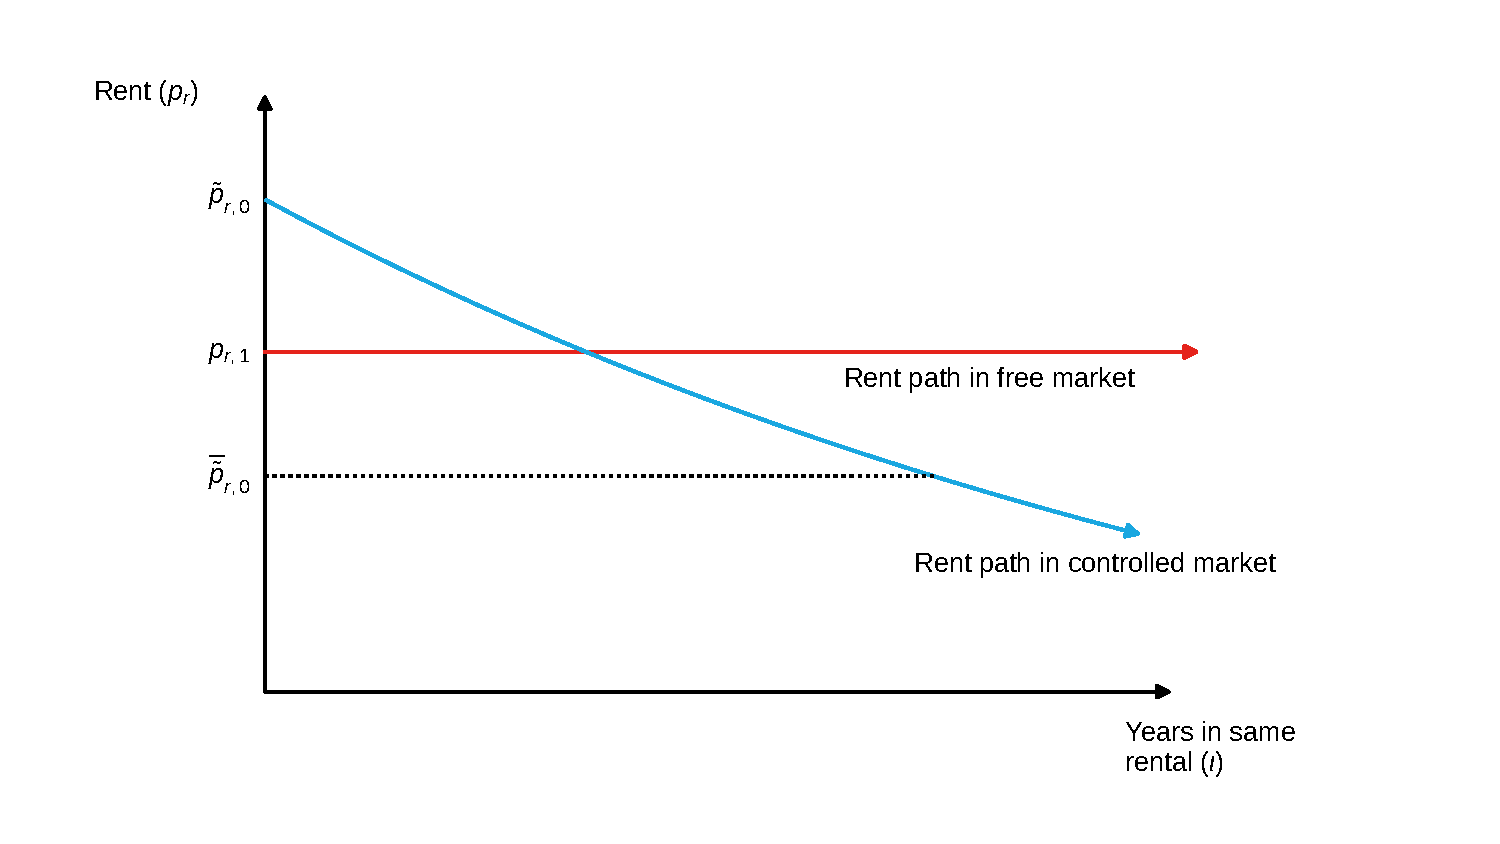
\includegraphics[width=\textwidth]{figures/path_of_rent_diagram.pdf}
    \vspace{-1.3cm}
    \begin{fignote2}{1.0\textwidth}
    \textit{Notes:} The downward-sloping blue line shows how rents decline over time for tenants in tenancy-controlled units, starting from the initial rent $\tilde{p}_{r,0}$ and averaging to $\overline{\tilde{p}}_{r,0}$. The horizontal red line represents the free-market rent, $p_{r,1}$. Free-market rents remain constant regardless of tenancy duration. Initially, controlled tenants pay more, but over time they benefit from lower rents. This ``entry premium'' deters short-term tenants, who prefer lower upfront costs, from choosing controlled units, while long-term tenants are willing to pay it for improved affordability later.
   \end{fignote2}
\end{figure}

\begin{figure}[H]
  \centering
    \caption{Lifecycle statistics}
    \vspace{-0.2cm}
    \label{fig:life_cycle}
    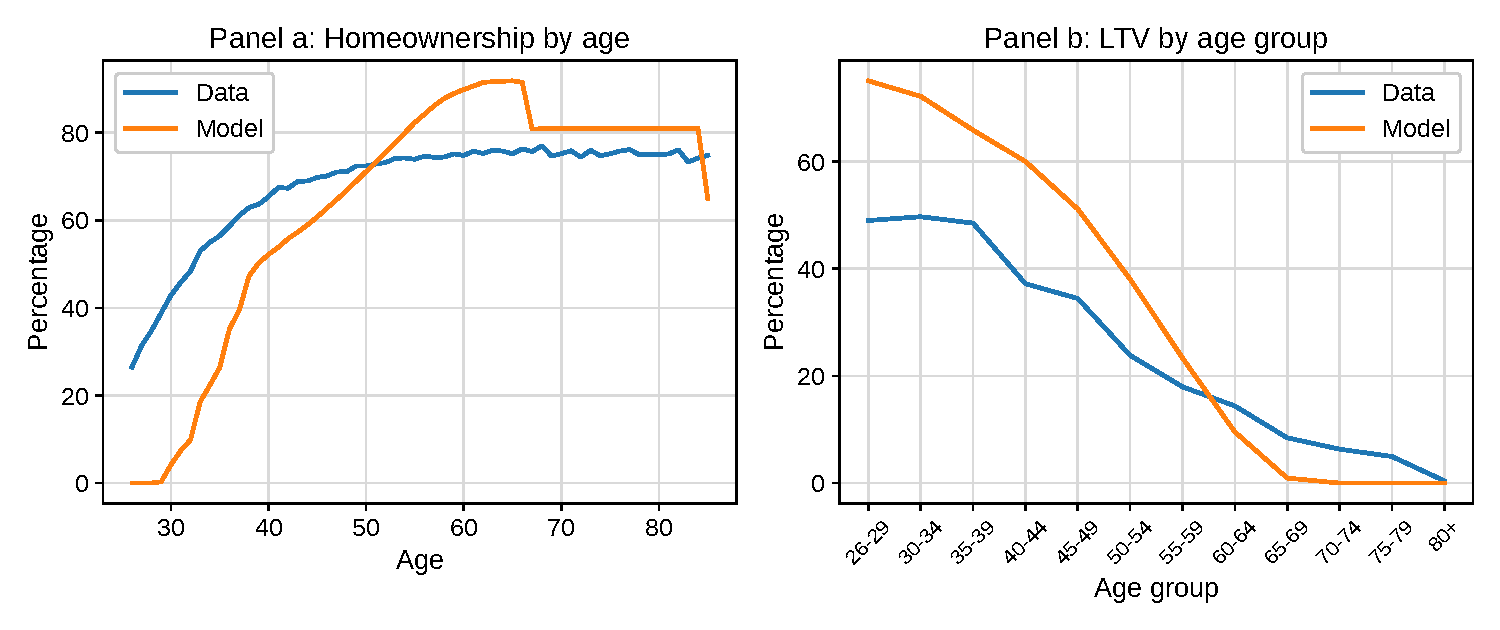
\includegraphics[width=\textwidth]{figures/homeownership_and_LTV.pdf}
    \vspace{-0.45cm}
    \begin{fignote2}{1\textwidth}
      \textit{Notes:} In Figure \ref{fig:life_cycle}, the two panels illustrate the model's performance on lifecycle statistics compared to the data. Panel (a) displays the average homeownership rate for each age cohort, while panel (b) presents the average loan-to-value (LTV) ratios for homeowners across 12 age groups, as the 2019 SFS provides household maintainers' ages in 5-year ranges. Model outputs are depicted in orange, while data are represented in blue. We source homeownership rates by age for Toronto CMA from the 2016 Census, and obtain data on the average LTV ratios from the 2019 SFS.
    \end{fignote2}
\end{figure}

\newpage

\appendix
% Number appendix equations (A.1), (A.2), ... as the EER Guide for Authors requires
\setcounter{equation}{0}
\renewcommand{\theequation}{\thesection.\arabic{equation}}
\setcounter{page}{1}
%\maketitle

\vspace{-3cm}
\noindent {\Large Online Appendix: ``Rent Control? Bad in Theory, Not Always in Practice''}

\section{Data and moment construction}\label{appendix:data}

In Section \ref{appendix:data} we describe some of the more complex variables we estimate, organized into rental market variables, income- and tax-related variables, and other variables. We compute all variables for the Toronto CMA. The exception is a subset of variables constructed using the 2019 Survey of Financial Security (SFS), for which we use Ontario data because the publicly available SFS identifies geography only down to the provincial level.

\subsection{Rental markets}\label{appendix:rental_markets}

\subsubsection{Percentage of renters in the controlled market}

To compute the percentage of renters residing in controlled units, we rely on data from the 2016 Census. We utilize the variable BUILT to distinguish between controlled and free-market units, subsequently dividing the total number of controlled units by the total number of rental units across both markets. This analysis reveals that 71\% of renters leased properties in the controlled market, implying that 29\% of renters opted for units in the free market. We denote the fraction of renters in the controlled market as $D$.

\subsubsection{Average number of years in a tenancy-controlled rental}

For our calibration, we need to estimate the ``entry premium'' in the controlled market. To compute this, we first need to know the average number of years a renter remains in the same rental. 

We estimate this using the average renter turnover rate of 12.25\% from the 2016--2021 RMS data sample. Utilizing this value, we compute the average number of years a renter stays in the same unit using the following formula:

\begin{equation}\label{eq:avg_tenure_duration}
    Y=\sum_{i=1}^{50}i\left[(1-\tau_{\text{turnover}})^{i-1}-(1-\tau_{\text{turnover}})^{i}\right].
\end{equation}

\noindent $Y$ represents the average number of years renters stay in the same unit, where $\tau_{\text{turnover}}$ denotes the turnover rate, and $i$ signifies the number of years.

To grasp the mechanics of equation \eqref{eq:avg_tenure_duration}, imagine an initial mass of renters equal to $1$. After one year, a fraction of $1-\tau_{\text{turnover}}$ remains in their unit, implying that a fraction of $\tau_{\text{turnover}}$ resides in their unit for precisely one year. After two years, a fraction of $(1-\tau_{\text{turnover}})^2$ continues to reside in their unit, suggesting that a fraction of $(1-\tau_{\text{turnover}})-(1-\tau_{\text{turnover}})^2$ resided in their unit for exactly two years, and so forth. We truncate the calculation at 50 years, as essentially no renters remain in the same unit for such an extended duration. By multiplying each fraction of renters living precisely $i$ years in the same unit by the number of years they resided in their unit, we obtain the expected number of years renters live in the same unit.

Next, using the estimated fraction of renters in the controlled market ($D$) and our approximation for the average number of years a renter is expected to stay in the same unit across both the controlled and free market ($Y$), we can derive the average number of years a renter in the controlled market remains in the same unit, $Y_{c}$, as follows:

\begin{equation*}
    Y_{c}=\frac{Y-(1-D)Y_{f}}{D}.
\end{equation*}

\noindent $Y_{f}$ denotes the average number of years a renter stays in a free market unit. To obtain $Y_{c}$, we leverage the estimate in \citet{cjq-2023} that renters in the controlled market remain in the same unit twice as long as renters in the free market, which implies that $Y_{f}=\frac{Y_{c}}{2}$. Thus, we can solve for $Y_{c}$, which is 9.55.

\subsubsection{Measuring ``entry premiums'' under tenancy control}\label{section:appendix_measuring_premium}

To estimate the ``entry premium'' paid by new tenants in controlled units relative to comparable units in the free market, we use household-level data from the 2016 Census. Our empirical strategy is to estimate average free-market rents based on observable unit characteristics (specifically the number of bedrooms (BEDRM) and unit condition (REPAIR)).

We identify new tenants in controlled units using the variables BUILT and MOB1, and then compute the percentage difference between the rent they pay and the quality-adjusted average free-market rent for comparable units. This difference represents the ``entry premium'' paid by new tenants in the controlled market. However, since controlled units systematically differ in quality from those in the free market, we need to adjust average free-market rents to account for these differences.

To do so, we draw on the estimates of \citet{zhang-gou}, who employ a regression discontinuity design (RDD) based on Toronto’s rent control exemption threshold. Comparing rental units completed just before and after the November 1, 1991 cutoff, they attribute only $13.7\%$ of the observed rent gap to direct effects of rent control, whereas $24.01\%$ of the gap reflects differences in unit quality, location, and amenities. We use these estimates to quality-adjust rents of controlled units. However, these quality differences include units of tenants who have lived in their units for a while, not newly occupied units. We thus adjust the quality to reflect the quality at the time of entry.

We do so by incorporating the model’s annual depreciation rate $\delta$ and average tenure duration $Y_{c}$. This captures the possibility that weaker maintenance incentives during regulated tenancies reduce quality over time. This yields the following quality-adjustment deflator for newly occupied controlled units:

\begin{equation}\label{eq:deflator}
    \text{Deflator}=1.2401-[(1+\delta)^{Y_c-1}-1].
\end{equation}

\noindent With our parameter values, this produces a deflator of $1.188$, which means that newly occupied controlled units are, on average, $18.8\%$ lower in quality than otherwise comparable free-market units, \emph{ceteris paribus}.

After applying this deflator to average free-market rents, we compute the ``entry premium'' paid by each new tenant in the controlled sector and then take the average. We estimate an average ``entry premium'' of $5.9\%$, with a $95\%$ confidence interval of $[2.7\%, 9.1\%]$.\footnote{If we do not apply this adjustment for controlled units of new tenants, the point estimate is about $10.5\%$ with a confidence interval of $[7.2\%,13.9\%]$. Thus, we view our estimate of $5.9\%$ for the ``entry premium'' as a conservative lower bound.}

\subsubsection{Age- and income-based discrimination under tenancy control}\label{section:appendix_discrimination}

We also examine whether landlords discriminate among new tenants in controlled units based on age or income. Using household-level data from the 2016 Census, we estimate the following regression:

\begin{equation*}
\text{SHELCO}_j = \alpha + \beta_1 i.\text{AGEGRP}_j + \beta_2 \text{TOTINC}_j + \beta_3 \text{BEDRM}_j + \beta_4 i.\text{REPAIR}_j + \beta_5 \text{ROOMS}_j, 
\end{equation*}

\noindent where the sample is restricted to new tenants in controlled units. %— defined as households for which is\_controlled$=1$ and is\_new\_tenant$=1$.

In this specification:

\begin{itemize} 
    \item $\text{SHELCO}_j$ is household $j$'s reported shelter cost. 
    \item $\text{AGEGRP}_j$ is a categorical variable indicating the age group the household head belongs to. 
    \item $\text{TOTINC}_j$ is the total pre-tax income of household $j$. 
    \item $\text{BEDRM}_j$ denotes the number of bedrooms in the rented unit of household $j$. 
    \item $\text{REPAIR}_j$ is a categorical variable indicating the unit’s state of repair. 
    \item $\text{ROOMS}_j$ represents the total number of rooms in household $j$'s unit. 
    \item $\beta_1$ and $\beta_4$ are vectors corresponding to the categorical variables $\text{AGEGRP}_j$ and $\text{REPAIR}_j$, respectively. 
\end{itemize}

The sample includes only households that moved into their unit within the past 12 months, identified by MOB1. Moreover, a unit is classified as rent-controlled if it was built before 1992, using the variable BUILT.

The regression results yield the following insights. None of the coefficients in $\beta_1$, corresponding to the age categories $\text{AGEGRP}_j$, are statistically significant at the 5\% level, indicating no evidence of age-based discrimination in initial rents. The coefficient on $\text{TOTINC}_j$, $\beta_2$, is statistically significant but small in magnitude with a value of 0.003. This implies that an increase of \$10,000 in total pre-tax income is associated with only a \$30 increase in initial rent, or approximately 2\% of the average initial controlled rent.

More importantly, this suggests that conditional on observables, higher-income renters face slightly higher initial rents than lower-income renters. From a policy perspective, this pattern is less concerning, as lower-income renters, who are the intended beneficiaries of rent control in most cases, do not appear to be disadvantaged. Instead, they may actually benefit from a somewhat preferential treatment in initial rent pricing.

\subsubsection{Rent-to-house-price ratio}

To calculate the rent-to-house price ratio, we use the average annual rent across all rental units in the 2006 RMS data, which was \$992 per month. Then, we multiply this figure by 12 and divide it by the average condo price in 2006, which was about \$227,000. The condo price data were combined in one place by Listings.ca for Toronto using several Toronto Real Estate Board (TREB) reports.\footnote{See \url{https://toronto.listing.ca/condo-price-history.htm}.} This computation results in a ratio of about $0.0524$.

\subsubsection{Rent-to-house-price ratio in free market}

To compute the rent-to-house price ratio in the free market, we utilize three estimated figures. Firstly, we have our computed rent-to-house price ratio across both markets, which is $0.0524$ as discussed just above. Secondly, in order to align with the year for which we computed the rent-to-price estimate above, we use 2006 Census data to estimate the share of the controlled market in the aggregate rental market, which was $D=87.62\%$. Thirdly, we incorporate an estimate from \citet{zhang-gou} regarding how much lower the average rent in the controlled market is relative to the average rent in the free market, all else being equal. We denote this difference as $T$. We formulate the rent-to-price ratio as follows:

\begin{equation}\label{eq:free_market_rent_to_price}
    {\left(\frac{\overline{p}_{r}}{p}\right)}=D \left(\frac{\overline{p}^{0}_{r}}{p}\right)+(1-D) \left(\frac{\overline{p}^{1}_{r}}{p}\right).
\end{equation}

\noindent $\left(\frac{\overline{p}_{r}}{p}\right)$ represents the rent-to-average price ratio, $\overline{p}^{0}_{r}$ denotes the average controlled rent, and $\overline{p}^{1}_{r}$ signifies the average free-market rent. Given that $\frac{\overline{p}^{0}_{r}}{p}=(1-T)\frac{\overline{p}^{1}_{r}}{p}$, we can substitute this into equation \eqref{eq:free_market_rent_to_price} and solve for $\frac{\overline{p}^{1}_{r}}{p}=0.0582$.

\subsubsection{Renters in the controlled market by income quintile}

Using 2016 Census data, we determine the percentage of households in each income quintile who rent in the controlled market. We categorize households into income quintiles using the total income variable (TOTINC), distinguish renters from owners using the tenure variable (TENUR), and identify controlled-market renters using the year-built variable (BUILT).

\subsection{Income and taxes}

\subsubsection{Increase in real average income by age}

To derive the deterministic age-related growth component of labor income, $\zeta_{j}$, we leverage data from the 2016 Census. Firstly, we calculate the average market income (EMPIN) for households whose household head's age ranged from 25 to 64 (AGEGRP). Subsequently, we regress income on age and age squared, as we outlined in Section \ref{sec:calibration}.

\subsubsection{Average income tax rate}

We calculate the average income tax rate based on data from the 2016 Census. This involved dividing total taxes paid (TOTINC - TOTINC\_AT) by total income (TOTINC). The resulting average income tax rate is 19.6\%.

\subsubsection{Estimating progressivity of income taxes}

In our model, we define income taxes by equation \eqref{eq:taxable_labor_income}. Rearranging this equation, we obtain:

\begin{equation}\label{eq:taxable_labor_income_regression}
  \mbox{log}(y^{x}_{j}(\chi,e,a)-y^{\tau}_{j}(\chi,e,a))=\mbox{log}(\tau_{\ell})+\psi \mbox{log}(y^{x}_{j}(\chi,e,a)).
\end{equation}

\noindent The left-hand side variable represents the log of after-tax taxable household income, while the right-hand side has an intercept and the log of taxable household income. The intercept is $\log(\tau_{\ell})$, and the coefficient on taxable household income is $\psi$, which determines the progressivity of income taxes. Regressing household-level 2016 Census data following equation \eqref{eq:taxable_labor_income_regression}, we obtain a point estimate for $\psi$ equal to 0.9275. Since taxes in the 2016 Census were not categorized by income type, we utilize after-tax household income from all sources and pre-tax household income from all sources.

\subsection{Other statistics}

\subsubsection{Property tax rate}

To calculate the property tax rate $\tau_p$, we draw on two data sources. Firstly, we rely on the property tax rate reported by the City of Toronto for 2023, which is 0.67\%.\footnote{See \url{https://www.toronto.ca/services-payments/property-taxes-utilities/property-tax/property-tax-rates-and-fees/2023-property-tax-rates-and-fees/}.} However, the property values assessed by municipalities in the City of Toronto often differ significantly from their actual values. Altus Group reports that more than 50\% of properties sold in Toronto in 2023 were assessed to be worth 35\% less than their actual sale price.\footnote{See page 12 here \url{https://assets.ctfassets.net/8jgyidtgyr4v/10K5oUs2wflXLjLgS8s44T/7dd2acc41dd82873f2e3e459f176e1f7/ENG_-_2024_Canadian_Tax_Rate_Benchmark_Report.pdf}.} Thus, this implies an effective property tax rate of $0.67\% \times 0.65 \approx 0.44\%$.

\subsubsection{Aggregate bequests to aggregate net wealth}

To compute the aggregate bequests to aggregate net wealth ratio, we use data from the 2019 SFS and the Life Tables for Canada, which we sourced from the World Health Organization.\footnote{See \url{apps.who.int/gho/data/view.searo.60290?lang=en}.} We calculate the net wealth for economic families within each age cohort (PWNETWPG) and then multiply this aggregate sum by the death rate of each age cohort. This process provides us with the total value of bequests for each age cohort. We sum up all bequests across all age cohorts and divide this total by the sum of net wealth for all economic families. As a result, we obtain a ratio of 0.022, indicating that aggregate bequests constitute 2.2\% of aggregate net wealth. This estimate aligns closely with figures reported for the United States (see \citet{cagetti-denardi-2006}).

\end{document}